% Options for packages loaded elsewhere
\PassOptionsToPackage{unicode}{hyperref}
\PassOptionsToPackage{hyphens}{url}
\PassOptionsToPackage{dvipsnames,svgnames,x11names}{xcolor}
%
\documentclass[
  letterpaper,
  DIV=11,
  numbers=noendperiod]{scrartcl}

\usepackage{amsmath,amssymb}
\usepackage{iftex}
\ifPDFTeX
  \usepackage[T1]{fontenc}
  \usepackage[utf8]{inputenc}
  \usepackage{textcomp} % provide euro and other symbols
\else % if luatex or xetex
  \usepackage{unicode-math}
  \defaultfontfeatures{Scale=MatchLowercase}
  \defaultfontfeatures[\rmfamily]{Ligatures=TeX,Scale=1}
\fi
\usepackage{lmodern}
\ifPDFTeX\else  
    % xetex/luatex font selection
\fi
% Use upquote if available, for straight quotes in verbatim environments
\IfFileExists{upquote.sty}{\usepackage{upquote}}{}
\IfFileExists{microtype.sty}{% use microtype if available
  \usepackage[]{microtype}
  \UseMicrotypeSet[protrusion]{basicmath} % disable protrusion for tt fonts
}{}
\makeatletter
\@ifundefined{KOMAClassName}{% if non-KOMA class
  \IfFileExists{parskip.sty}{%
    \usepackage{parskip}
  }{% else
    \setlength{\parindent}{0pt}
    \setlength{\parskip}{6pt plus 2pt minus 1pt}}
}{% if KOMA class
  \KOMAoptions{parskip=half}}
\makeatother
\usepackage{xcolor}
\setlength{\emergencystretch}{3em} % prevent overfull lines
\setcounter{secnumdepth}{5}
% Make \paragraph and \subparagraph free-standing
\ifx\paragraph\undefined\else
  \let\oldparagraph\paragraph
  \renewcommand{\paragraph}[1]{\oldparagraph{#1}\mbox{}}
\fi
\ifx\subparagraph\undefined\else
  \let\oldsubparagraph\subparagraph
  \renewcommand{\subparagraph}[1]{\oldsubparagraph{#1}\mbox{}}
\fi

\usepackage{color}
\usepackage{fancyvrb}
\newcommand{\VerbBar}{|}
\newcommand{\VERB}{\Verb[commandchars=\\\{\}]}
\DefineVerbatimEnvironment{Highlighting}{Verbatim}{commandchars=\\\{\}}
% Add ',fontsize=\small' for more characters per line
\usepackage{framed}
\definecolor{shadecolor}{RGB}{241,243,245}
\newenvironment{Shaded}{\begin{snugshade}}{\end{snugshade}}
\newcommand{\AlertTok}[1]{\textcolor[rgb]{0.68,0.00,0.00}{#1}}
\newcommand{\AnnotationTok}[1]{\textcolor[rgb]{0.37,0.37,0.37}{#1}}
\newcommand{\AttributeTok}[1]{\textcolor[rgb]{0.40,0.45,0.13}{#1}}
\newcommand{\BaseNTok}[1]{\textcolor[rgb]{0.68,0.00,0.00}{#1}}
\newcommand{\BuiltInTok}[1]{\textcolor[rgb]{0.00,0.23,0.31}{#1}}
\newcommand{\CharTok}[1]{\textcolor[rgb]{0.13,0.47,0.30}{#1}}
\newcommand{\CommentTok}[1]{\textcolor[rgb]{0.37,0.37,0.37}{#1}}
\newcommand{\CommentVarTok}[1]{\textcolor[rgb]{0.37,0.37,0.37}{\textit{#1}}}
\newcommand{\ConstantTok}[1]{\textcolor[rgb]{0.56,0.35,0.01}{#1}}
\newcommand{\ControlFlowTok}[1]{\textcolor[rgb]{0.00,0.23,0.31}{#1}}
\newcommand{\DataTypeTok}[1]{\textcolor[rgb]{0.68,0.00,0.00}{#1}}
\newcommand{\DecValTok}[1]{\textcolor[rgb]{0.68,0.00,0.00}{#1}}
\newcommand{\DocumentationTok}[1]{\textcolor[rgb]{0.37,0.37,0.37}{\textit{#1}}}
\newcommand{\ErrorTok}[1]{\textcolor[rgb]{0.68,0.00,0.00}{#1}}
\newcommand{\ExtensionTok}[1]{\textcolor[rgb]{0.00,0.23,0.31}{#1}}
\newcommand{\FloatTok}[1]{\textcolor[rgb]{0.68,0.00,0.00}{#1}}
\newcommand{\FunctionTok}[1]{\textcolor[rgb]{0.28,0.35,0.67}{#1}}
\newcommand{\ImportTok}[1]{\textcolor[rgb]{0.00,0.46,0.62}{#1}}
\newcommand{\InformationTok}[1]{\textcolor[rgb]{0.37,0.37,0.37}{#1}}
\newcommand{\KeywordTok}[1]{\textcolor[rgb]{0.00,0.23,0.31}{#1}}
\newcommand{\NormalTok}[1]{\textcolor[rgb]{0.00,0.23,0.31}{#1}}
\newcommand{\OperatorTok}[1]{\textcolor[rgb]{0.37,0.37,0.37}{#1}}
\newcommand{\OtherTok}[1]{\textcolor[rgb]{0.00,0.23,0.31}{#1}}
\newcommand{\PreprocessorTok}[1]{\textcolor[rgb]{0.68,0.00,0.00}{#1}}
\newcommand{\RegionMarkerTok}[1]{\textcolor[rgb]{0.00,0.23,0.31}{#1}}
\newcommand{\SpecialCharTok}[1]{\textcolor[rgb]{0.37,0.37,0.37}{#1}}
\newcommand{\SpecialStringTok}[1]{\textcolor[rgb]{0.13,0.47,0.30}{#1}}
\newcommand{\StringTok}[1]{\textcolor[rgb]{0.13,0.47,0.30}{#1}}
\newcommand{\VariableTok}[1]{\textcolor[rgb]{0.07,0.07,0.07}{#1}}
\newcommand{\VerbatimStringTok}[1]{\textcolor[rgb]{0.13,0.47,0.30}{#1}}
\newcommand{\WarningTok}[1]{\textcolor[rgb]{0.37,0.37,0.37}{\textit{#1}}}

\providecommand{\tightlist}{%
  \setlength{\itemsep}{0pt}\setlength{\parskip}{0pt}}\usepackage{longtable,booktabs,array}
\usepackage{calc} % for calculating minipage widths
% Correct order of tables after \paragraph or \subparagraph
\usepackage{etoolbox}
\makeatletter
\patchcmd\longtable{\par}{\if@noskipsec\mbox{}\fi\par}{}{}
\makeatother
% Allow footnotes in longtable head/foot
\IfFileExists{footnotehyper.sty}{\usepackage{footnotehyper}}{\usepackage{footnote}}
\makesavenoteenv{longtable}
\usepackage{graphicx}
\makeatletter
\def\maxwidth{\ifdim\Gin@nat@width>\linewidth\linewidth\else\Gin@nat@width\fi}
\def\maxheight{\ifdim\Gin@nat@height>\textheight\textheight\else\Gin@nat@height\fi}
\makeatother
% Scale images if necessary, so that they will not overflow the page
% margins by default, and it is still possible to overwrite the defaults
% using explicit options in \includegraphics[width, height, ...]{}
\setkeys{Gin}{width=\maxwidth,height=\maxheight,keepaspectratio}
% Set default figure placement to htbp
\makeatletter
\def\fps@figure{htbp}
\makeatother

% load packages
\usepackage{geometry}
\usepackage{xcolor}
\usepackage{eso-pic}
\usepackage{fancyhdr}
\usepackage{sectsty}
\usepackage{fontspec}
\usepackage{titlesec}

%% Set page size with a wider right margin
\geometry{a4paper, total={170mm,257mm}, left=20mm, top=20mm, bottom=20mm, right=50mm}

%% Let's define some colours
\definecolor{uniblue}{HTML}{003865}
\definecolor{burgundy}{HTML}{7D2239}
\definecolor{cobalt}{HTML}{005C8A}
\definecolor{lavender}{HTML}{5B4D94}
\definecolor{leaf}{HTML}{006630}
\definecolor{moss}{HTML}{385A4F}
\definecolor{pillarbox}{HTML}{B30C00}
\definecolor{rust}{HTML}{9A3A06}
\definecolor{sandstone}{HTML}{52473B}
\definecolor{skyblue}{HTML}{005398}
\definecolor{slate}{HTML}{4F5961}
\definecolor{thistle}{HTML}{951272}

%\definecolor{light}{HTML}{E6E6FA} % original from template - redefined below as uni blue at 10 percent:
\colorlet{light}{uniblue!10}
%\definecolor{highlight}{HTML}{800080} % original from template - redefined below as uni's skyblue:
\colorlet{highlight}{skyblue}
%\definecolor{dark}{HTML}{330033} % original from template - redefined below as uni blue at 100 percent:
\colorlet{dark}{uniblue}

%% Let's add the border on the right hand side 
\AddToShipoutPicture{% 
    \AtPageLowerLeft{% 
        \put(\LenToUnit{\dimexpr\paperwidth-3cm},0){% 
            \color{light}\rule{3cm}{\LenToUnit\paperheight}%
          }%
     }%
     % logo
    \AtPageLowerLeft{% start the bar at the bottom right of the page
        \put(\LenToUnit{\dimexpr\paperwidth-2.25cm},27.2cm){% move it to the top right
            \color{light}
\includegraphics[width=2.25cm]{_extensions/nrennie/PrettyPDF/uni_logo_boxed.jpg}
          }%
     }%
}

%% Style the page number
\fancypagestyle{mystyle}{
  \fancyhf{}
  \renewcommand\headrulewidth{0pt}
  \fancyfoot[R]{\thepage}
  \fancyfootoffset{3.5cm}
}
\setlength{\footskip}{20pt}

%% style the chapter/section fonts
\chapterfont{\color{uniblue}\fontsize{20}{16.8}\selectfont}
\sectionfont{\color{uniblue}\fontsize{20}{16.8}\selectfont}
\subsectionfont{\color{skyblue}\fontsize{14}{16.8}\selectfont}
\titleformat{\subsection}
  {\color{uniblue!90}\sffamily\Large\bfseries}{\thesubsection}{1em}{}[{\titlerule[0.8pt]}]
\subsubsectionfont{\color{cobalt}}

\renewcommand\thesection{\color{slate}\arabic{section}}
  
% left align title
\makeatletter
\renewcommand{\maketitle}{\bgroup\setlength{\parindent}{0pt}
\begin{flushleft}
  {\color{uniblue}\sffamily\huge\textbf{\@title}} \vspace{0.3cm} \newline
  {\Large {\@subtitle}} \newline
  \@author
\end{flushleft}\egroup
}
\makeatother

%% Use some custom fonts
\setsansfont{Ubuntu}[
    Path=_extensions/nrennie/PrettyPDF/Ubuntu/,
    Scale=0.9,
    Extension = .ttf,
    UprightFont=*-Regular,
    BoldFont=*-Bold,
    ItalicFont=*-Italic,
    ]

\setmainfont{Ubuntu}[
    Path=_extensions/nrennie/PrettyPDF/Ubuntu/,
    Scale=0.9,
    Extension = .ttf,
    UprightFont=*-Regular,
    BoldFont=*-Bold,
    ItalicFont=*-Italic,
    ]
\usepackage{booktabs}
\usepackage{longtable}
\usepackage{array}
\usepackage{multirow}
\usepackage{wrapfig}
\usepackage{float}
\usepackage{colortbl}
\usepackage{pdflscape}
\usepackage{tabu}
\usepackage{threeparttable}
\usepackage{threeparttablex}
\usepackage[normalem]{ulem}
\usepackage{makecell}
\usepackage{xcolor}
\KOMAoption{captions}{tableheading}
\makeatletter
\@ifpackageloaded{tcolorbox}{}{\usepackage[skins,breakable]{tcolorbox}}
\@ifpackageloaded{fontawesome5}{}{\usepackage{fontawesome5}}
\definecolor{quarto-callout-color}{HTML}{909090}
\definecolor{quarto-callout-note-color}{HTML}{0758E5}
\definecolor{quarto-callout-important-color}{HTML}{CC1914}
\definecolor{quarto-callout-warning-color}{HTML}{EB9113}
\definecolor{quarto-callout-tip-color}{HTML}{00A047}
\definecolor{quarto-callout-caution-color}{HTML}{FC5300}
\definecolor{quarto-callout-color-frame}{HTML}{acacac}
\definecolor{quarto-callout-note-color-frame}{HTML}{4582ec}
\definecolor{quarto-callout-important-color-frame}{HTML}{d9534f}
\definecolor{quarto-callout-warning-color-frame}{HTML}{f0ad4e}
\definecolor{quarto-callout-tip-color-frame}{HTML}{02b875}
\definecolor{quarto-callout-caution-color-frame}{HTML}{fd7e14}
\makeatother
\makeatletter
\@ifpackageloaded{caption}{}{\usepackage{caption}}
\AtBeginDocument{%
\ifdefined\contentsname
  \renewcommand*\contentsname{Table of contents}
\else
  \newcommand\contentsname{Table of contents}
\fi
\ifdefined\listfigurename
  \renewcommand*\listfigurename{List of Figures}
\else
  \newcommand\listfigurename{List of Figures}
\fi
\ifdefined\listtablename
  \renewcommand*\listtablename{List of Tables}
\else
  \newcommand\listtablename{List of Tables}
\fi
\ifdefined\figurename
  \renewcommand*\figurename{Figure}
\else
  \newcommand\figurename{Figure}
\fi
\ifdefined\tablename
  \renewcommand*\tablename{Table}
\else
  \newcommand\tablename{Table}
\fi
}
\@ifpackageloaded{float}{}{\usepackage{float}}
\floatstyle{ruled}
\@ifundefined{c@chapter}{\newfloat{codelisting}{h}{lop}}{\newfloat{codelisting}{h}{lop}[chapter]}
\floatname{codelisting}{Listing}
\newcommand*\listoflistings{\listof{codelisting}{List of Listings}}
\makeatother
\makeatletter
\makeatother
\makeatletter
\@ifpackageloaded{caption}{}{\usepackage{caption}}
\@ifpackageloaded{subcaption}{}{\usepackage{subcaption}}
\makeatother
\makeatletter
\@ifpackageloaded{tcolorbox}{}{\usepackage[skins,breakable]{tcolorbox}}
\makeatother
\makeatletter
\@ifundefined{shadecolor}{\definecolor{shadecolor}{rgb}{.97, .97, .97}}{}
\makeatother
\makeatletter
\@ifundefined{codebgcolor}{\definecolor{codebgcolor}{named}{light}}{}
\makeatother
\makeatletter
\ifdefined\Shaded\renewenvironment{Shaded}{\begin{tcolorbox}[boxrule=0pt, frame hidden, sharp corners, enhanced, colback={codebgcolor}, breakable]}{\end{tcolorbox}}\fi
\makeatother
\ifLuaTeX
  \usepackage{selnolig}  % disable illegal ligatures
\fi
\usepackage{bookmark}

\IfFileExists{xurl.sty}{\usepackage{xurl}}{} % add URL line breaks if available
\urlstyle{same} % disable monospaced font for URLs
\hypersetup{
  pdftitle={Introduction to Quarto},
  colorlinks=true,
  linkcolor={highlight},
  filecolor={Maroon},
  citecolor={Blue},
  urlcolor={highlight},
  pdfcreator={LaTeX via pandoc}}

\title{Introduction to Quarto}
\author{}
\date{}

\begin{document}
\maketitle

\pagestyle{mystyle}

\renewcommand*\contentsname{Contents}
{
\hypersetup{linkcolor=}
\setcounter{tocdepth}{3}
\tableofcontents
}
\section{Introduction}\label{introduction}

This week we will take what we will produce a report using Quarto .
Quarto is a multi-language system that allows reports and presentation
to be created within R, thus allowing for R code and output to be easily
embedded within a report, a presentation or even a Blog! Hence, all of
the R code and plots obtained from an analysis are contained within a
single file.

Below you can download an example of a report produced with Quarto
relating to fitting a regression model. You can toggle the
\texttt{\textless{}/\textgreater{}\ Code} button in the html file to see
the source code that produced this file. It is advised to have this
document open while working through the remaining sections in order to
see examples put into practice.

The following sections will take you through the different steps
required to produce this report in Quarto. For creating a new Quarto
file from scratch see Section~\ref{sec-quarto_init}, otherwise move onto
Section~\ref{sec-title}.

\section{Creating your first Quarto document}\label{sec-quarto_init}

If you want to create a new Quarto document from scratch within RStudio
you can click on on the \texttt{New\ File} icon

\includegraphics[width=0.23958in,height=\textheight]{images/new_doc.png}
or go to:

\texttt{File\ -\textgreater{}\ New\ File\ -\textgreater{}\ Quarto\ \ Document...}

This will open the following window within RStudio:

\begin{center}
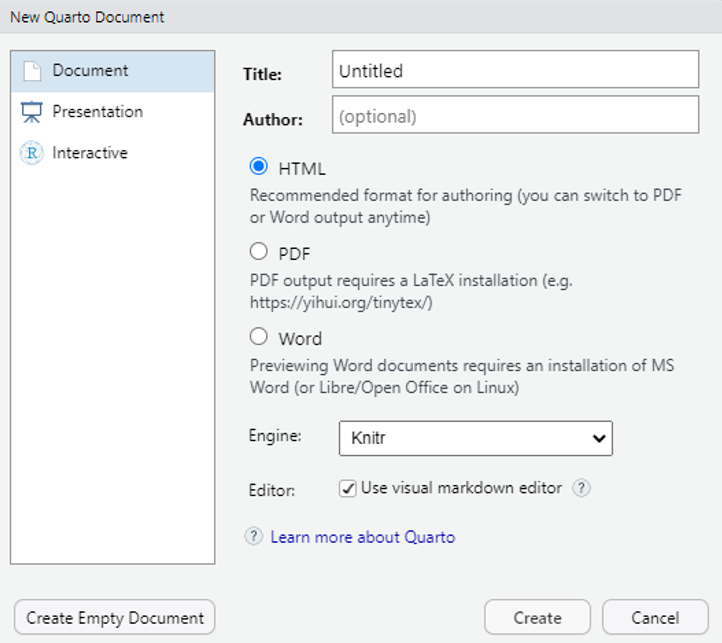
\includegraphics[width=5.20833in,height=\textheight]{images/quarto1.png}
\end{center}

\begin{tcolorbox}[enhanced jigsaw, left=2mm, toprule=.15mm, title=\textcolor{quarto-callout-important-color}{\faExclamation}\hspace{0.5em}{Important}, colbacktitle=quarto-callout-important-color!10!white, toptitle=1mm, titlerule=0mm, breakable, opacityback=0, bottomrule=.15mm, coltitle=black, arc=.35mm, rightrule=.15mm, bottomtitle=1mm, colframe=quarto-callout-important-color-frame, leftrule=.75mm, opacitybacktitle=0.6, colback=white]

If you are working on your personal computer be sure that you have the
latest RStudio
\href{https://posit.co/download/rstudio-desktop/}{version} installed.

\end{tcolorbox}

From here, select \textbf{Document} and the \textbf{Default Output
Format} as \textbf{HTML} (\textbf{PDF} output is also possible but you
need the latest version of \texttt{MikTex} to be installed if you are a
Windows user). Give your document a title and select OK. This will open
in RStudio an empty \texttt{.qmd} file.

\section{Title}\label{sec-title}

The title of the document can be found at the top of the \texttt{.qmd}
file within its \textbf{preamble} (YAML heading), which is shown below.
When titling your document, ensure the title is within inverted commas.

\begin{Shaded}
\begin{Highlighting}[]
\SpecialCharTok{{-}{-}{-}}
\NormalTok{title}\SpecialCharTok{:} \StringTok{"Data Analysis: Example Report"}
\SpecialCharTok{{-}{-}{-}}
\end{Highlighting}
\end{Shaded}

A Quarto document can be edited in the two modes of the RStudio editor:
visual (on the left) and source (on the right). The visual mode offers a
more friendly interface for editing you document (it includes a toolbar
for quick edit options), while the source mode allows you to see and
edit the underlying markdown text code.

\begin{center}
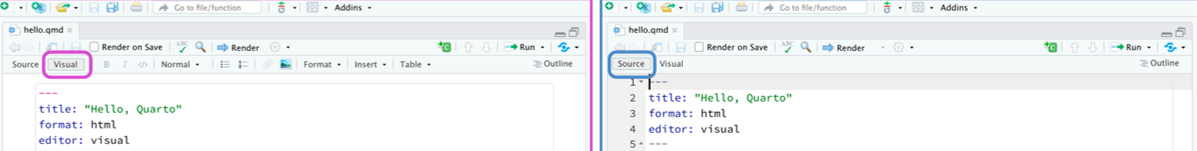
\includegraphics[width=7.94792in,height=\textheight]{images/quarto2.png}
\end{center}

You can switch between these two modes at anytime. We will now cover
different aspects of building a Quarto document and provide the
instructions on how to do this using either the visual editor or the
source mode.

\section{Sections}\label{sec-sections}

The structure of you quarto document can be determine by the different
sections contained in it.

Under the \texttt{source} mode, sections within a Quarto document are
created using \texttt{\#}. For example, \texttt{\#\ Introduction} will
create a section titled \textbf{Introduction}. Alternatively, if you use
the \texttt{visual} mode, you can include a new section by selecting a
proper heading under the block-format display of the toolbar as follows:

\begin{center}
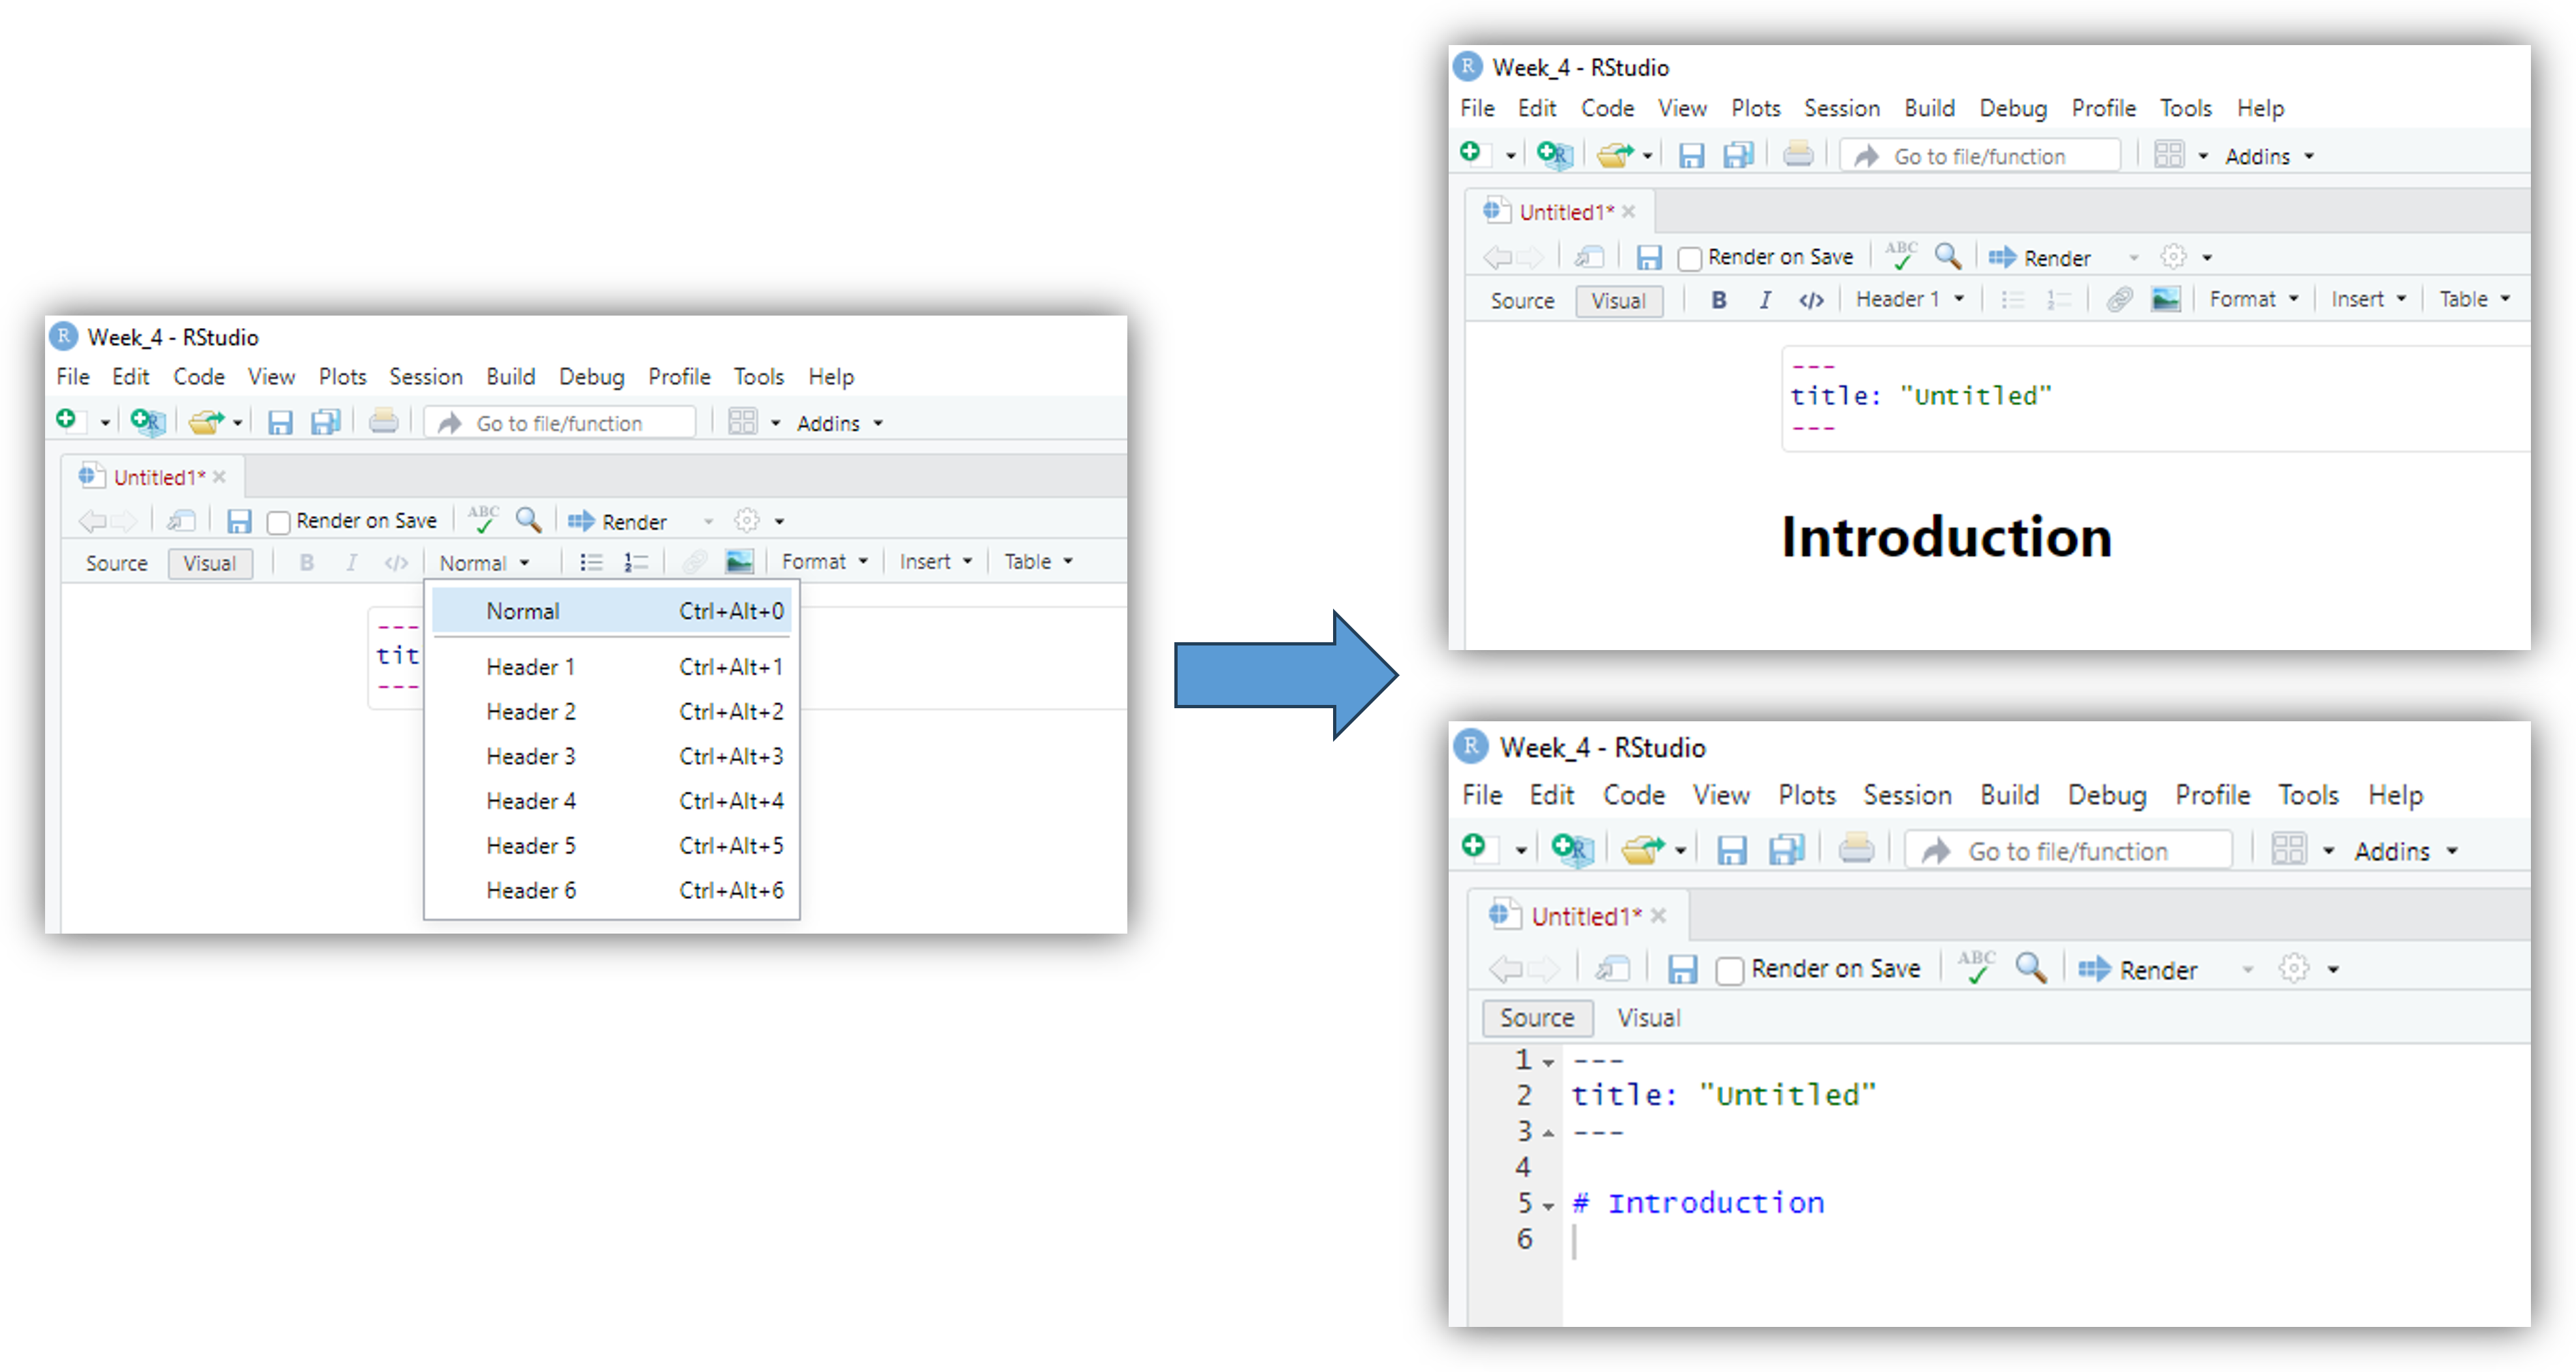
\includegraphics[width=7.64583in,height=\textheight]{images/quarto3.png}
\end{center}

If you want section to be numbered you can set
\texttt{number\_sections:\ true} within the preamble of the document:

\begin{Shaded}
\begin{Highlighting}[]
\SpecialCharTok{{-}{-}{-}}
\NormalTok{title}\SpecialCharTok{:} \StringTok{"Data Analysis: Example Report"}
\NormalTok{number}\SpecialCharTok{{-}}\NormalTok{sections}\SpecialCharTok{:}\NormalTok{ true}
\SpecialCharTok{{-}{-}{-}}
\end{Highlighting}
\end{Shaded}

\begin{tcolorbox}[enhanced jigsaw, left=2mm, toprule=.15mm, title={Task 1}, colbacktitle=quarto-callout-warning-color!10!white, toptitle=1mm, titlerule=0mm, breakable, opacityback=0, bottomrule=.15mm, coltitle=black, arc=.35mm, rightrule=.15mm, bottomtitle=1mm, colframe=quarto-callout-warning-color-frame, leftrule=.75mm, opacitybacktitle=0.6, colback=white]

Create a new quarto document by clicking on the \texttt{New\ File} icon

\includegraphics[width=0.23958in,height=\textheight]{images/new_doc.png}
, change the title to \emph{``Data Analysis: Example Report''} and add
numbered-level 1 headings for each of the following project sections:

\begin{itemize}
\item
  Introduction
\item
  Exploratory data analysis
\item
  Formal data analysis
\item
  Conclusions
\item
  References
\end{itemize}

Then, click the

\includegraphics[width=0.25in,height=0.20833in]{images/rstudio-render-button.png}\texttt{Render}
button and compile your Quarto document to make sure that your markdown
formatting produces the expected output in your HTML document.

Tip: Try typing \texttt{/} symbol on your main document while using the
visual mode and then use the drop menu to add a new section to your
document (you can type the letter \texttt{h} to search for the different
header types while the drop menu is being displayed).

See solution

Your quarto document should look like this if you go to the
\texttt{source\ mode}:

\begin{Shaded}
\begin{Highlighting}[]
\SpecialCharTok{{-}{-}{-}}
\NormalTok{title}\SpecialCharTok{:} \StringTok{"Data Analysis: Example Report"}
\NormalTok{number}\SpecialCharTok{{-}}\NormalTok{sections}\SpecialCharTok{:}\NormalTok{ true}
\SpecialCharTok{{-}{-}{-}}

\CommentTok{\# Introduction}

\CommentTok{\# Exploratory data analysis}

\CommentTok{\# Formal data analysis}

\CommentTok{\# Conclusions}

\CommentTok{\# References}
\end{Highlighting}
\end{Shaded}

\end{tcolorbox}

Each section can be assigned labels so that they can be referred to
within the text.

\section{\texorpdfstring{\texttt{visual} mode}{visual mode}}

For the \texttt{visual} model you can click on the edit attributes
settings

\includegraphics[width=0.17708in,height=\textheight]{images/threedots.png}
(right hand side of the section heading) and write the label you want on
the ID box of the pop-up window:

\begin{center}
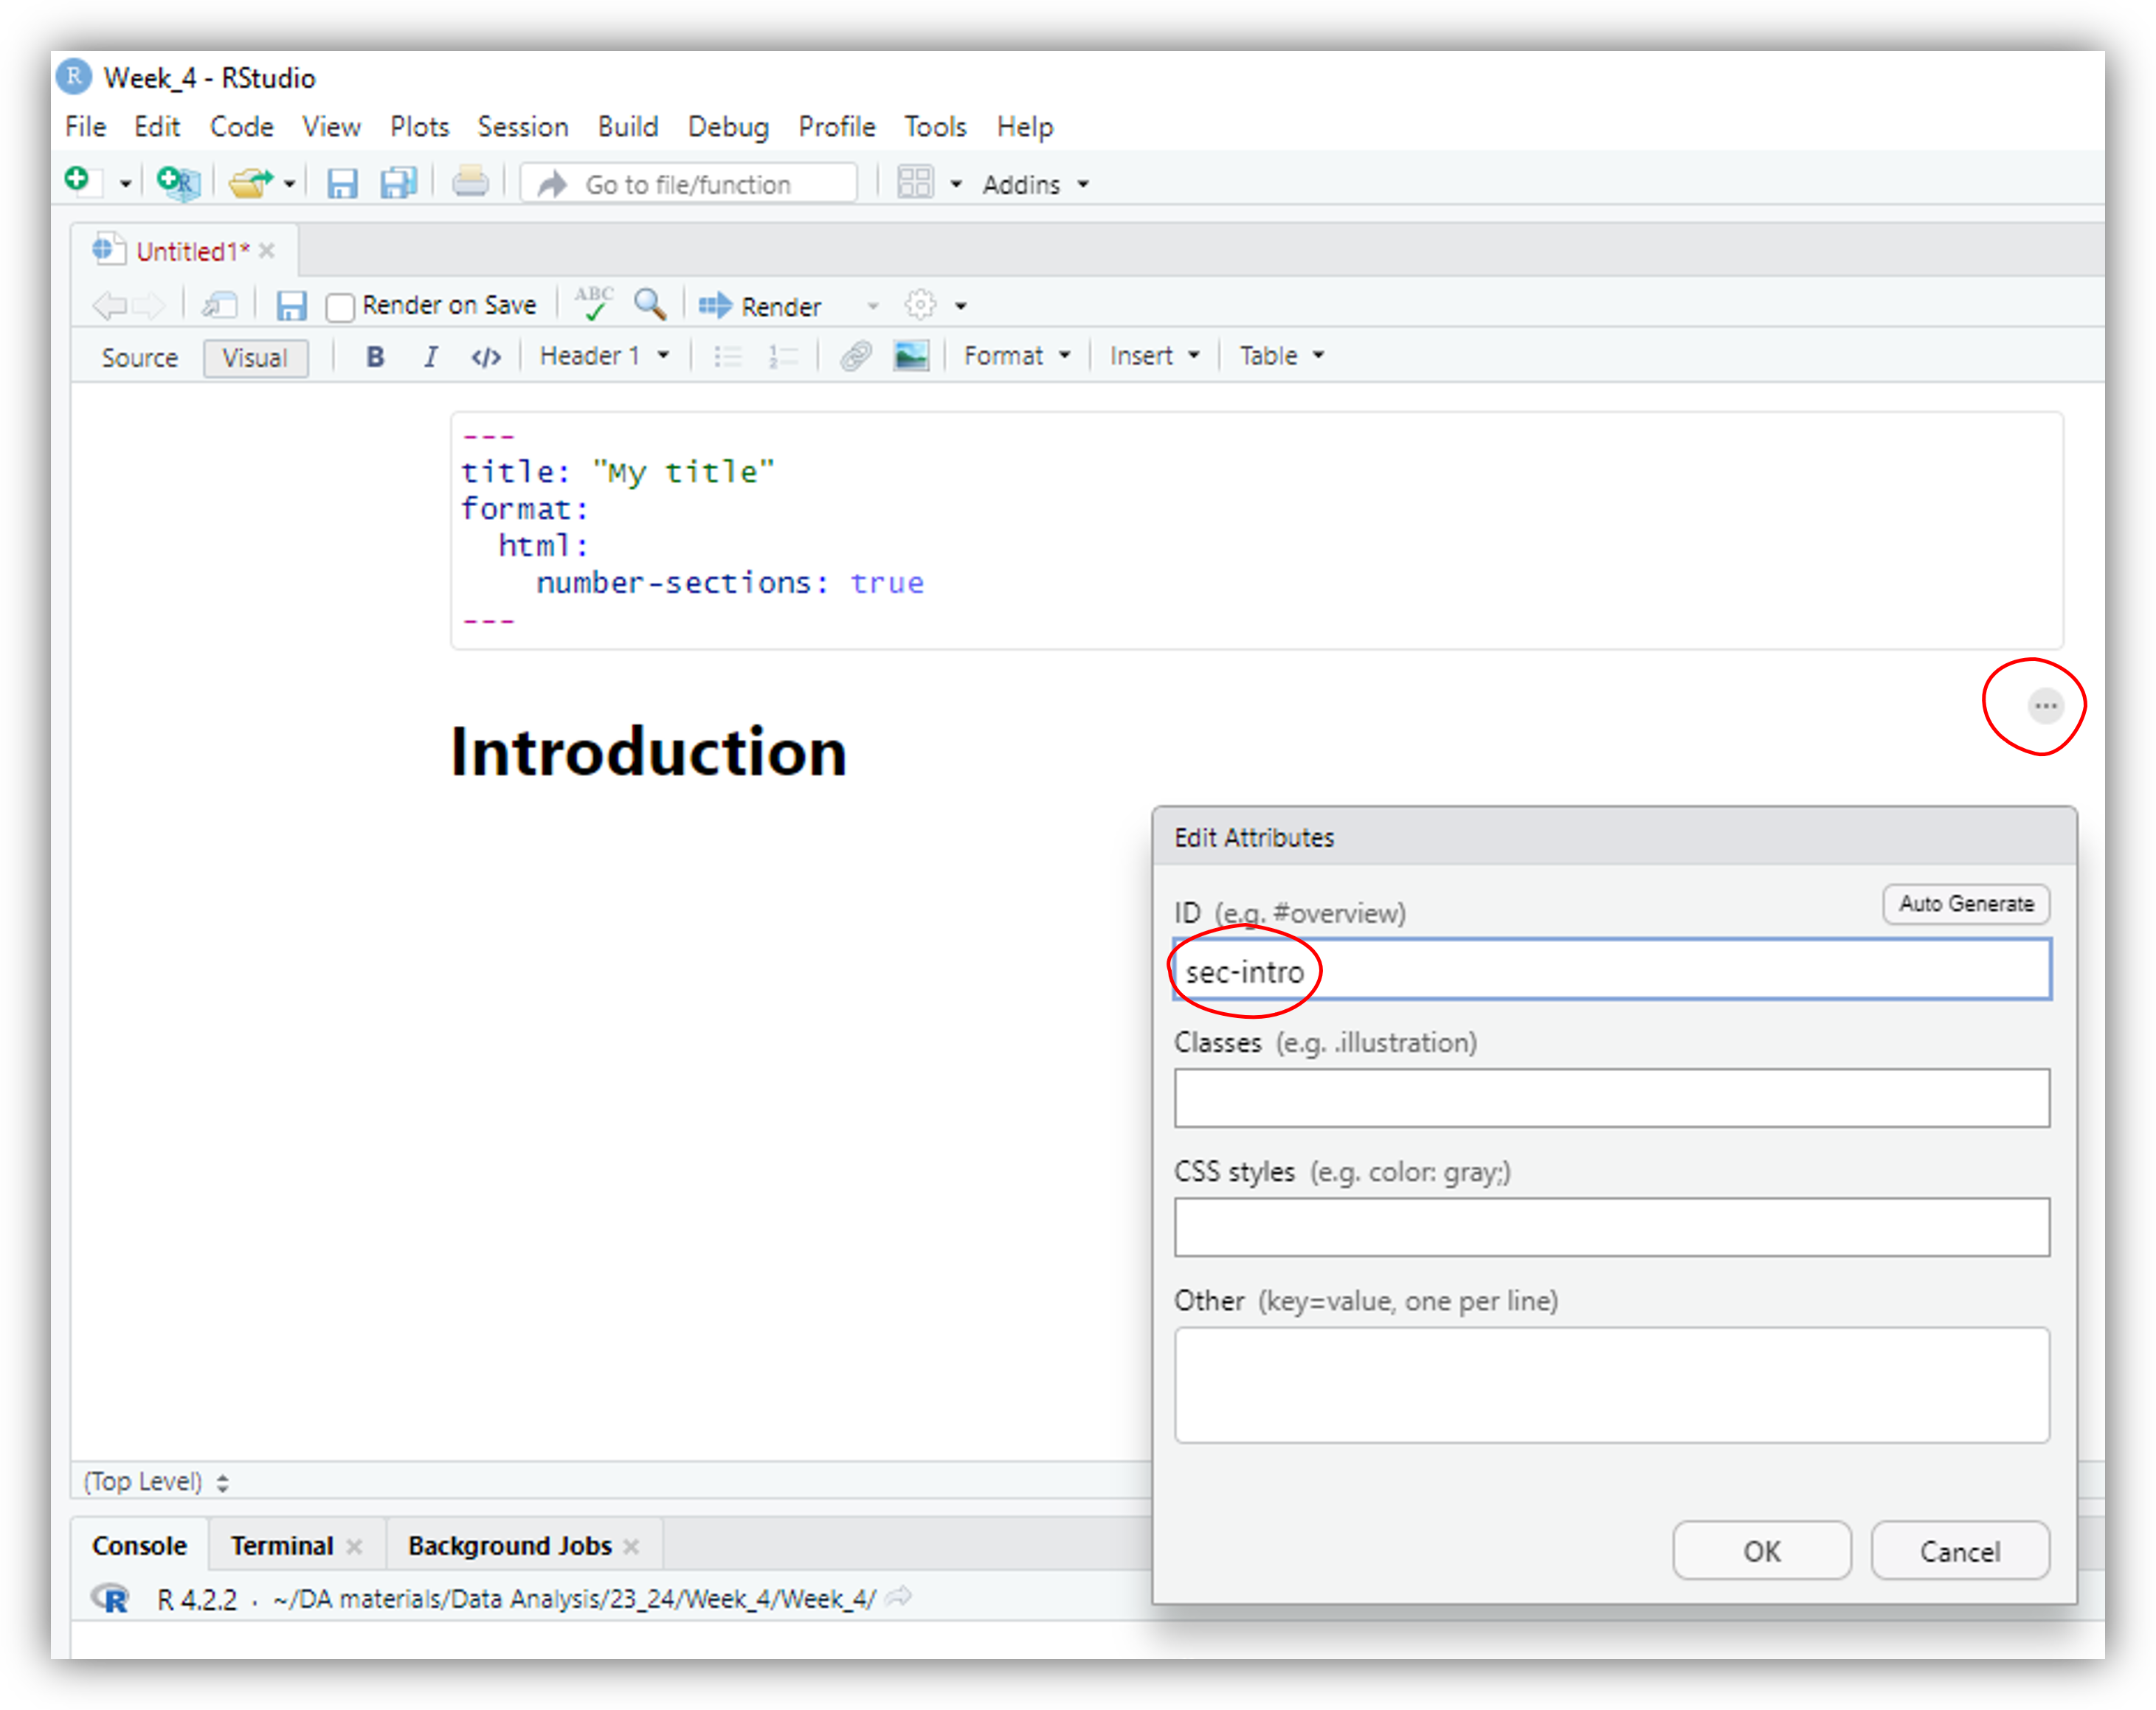
\includegraphics[width=5.39583in,height=\textheight]{images/quarto4.png}
\end{center}

\section{\texorpdfstring{\texttt{source} mode}{source mode}}

To reference a section, add a~\texttt{\#sec-}~identifier to any heading.
For example, to give our \textbf{Introduction} section a label we simply
add the label \texttt{\{\#sec-intro\}} to the section title as follows:

\begin{Shaded}
\begin{Highlighting}[]
\CommentTok{\# Introduction \{\#sec{-}intro\}}
\end{Highlighting}
\end{Shaded}

where \texttt{sec-intro} is the label chosen for this particular
section.

\begin{tcolorbox}[enhanced jigsaw, left=2mm, toprule=.15mm, title=\textcolor{quarto-callout-important-color}{\faExclamation}\hspace{0.5em}{Important}, colbacktitle=quarto-callout-important-color!10!white, toptitle=1mm, titlerule=0mm, breakable, opacityback=0, bottomrule=.15mm, coltitle=black, arc=.35mm, rightrule=.15mm, bottomtitle=1mm, colframe=quarto-callout-important-color-frame, leftrule=.75mm, opacitybacktitle=0.6, colback=white]

It is a good idea to label your sections appropriately so that it is
easy to refer to them later. Note that it is important to add the
\texttt{sec-} prefix in order for cross-referencing to work properly.

\end{tcolorbox}

The section can now be referred to within the text of the document using
the \texttt{@}sec- command. That is

\begin{Shaded}
\begin{Highlighting}[]
\SpecialCharTok{@}\NormalTok{sec}\SpecialCharTok{{-}}\NormalTok{intro ...}
\end{Highlighting}
\end{Shaded}

will produce

\begin{Shaded}
\begin{Highlighting}[]
\NormalTok{Section }\DecValTok{1}\NormalTok{ ...}
\end{Highlighting}
\end{Shaded}

where the 1 is a clickable hyperlink that will take you to the beginning
of that section within the document. If you are using the
\texttt{visual} mode, you can also easily include cross-references by
typing \texttt{@} and then scroll through the different hyperlinks you
created, or by clicking on \texttt{Insert▾➠\ Cross\ Reference}

Note that for section labels to appear on the references list, you must
save your document first (click on \texttt{File\ ➠\ Save\ as…} and save
your document with a proper name). Then all the labels (i.e., labels of
sections, figures, equations, etc.) will appear on the Insert Cross
Reference pop up window. Then simply click on \texttt{Insert▾} to add
the selected reference to your document:

\begin{center}
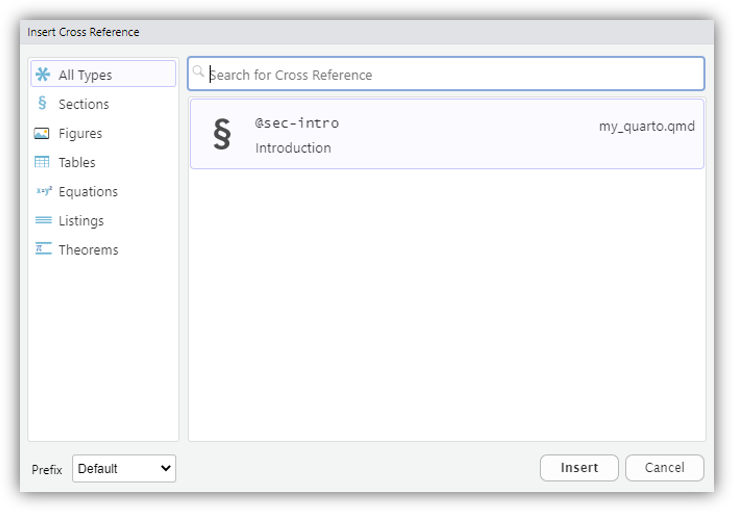
\includegraphics[width=5.5in,height=\textheight]{images/quarto5.png}
\end{center}

\begin{tcolorbox}[enhanced jigsaw, left=2mm, toprule=.15mm, title=\textcolor{quarto-callout-note-color}{\faInfo}\hspace{0.5em}{Note}, colbacktitle=quarto-callout-note-color!10!white, toptitle=1mm, titlerule=0mm, breakable, opacityback=0, bottomrule=.15mm, coltitle=black, arc=.35mm, rightrule=.15mm, bottomtitle=1mm, colframe=quarto-callout-note-color-frame, leftrule=.75mm, opacitybacktitle=0.6, colback=white]

Subsections can be added to a document in a similar fashion using either
\texttt{\#\#} (such that \texttt{\#\#\ Subsection\ \{\#sec-sub\}} will
create a subsection with the label \texttt{sec-sub} and title
\textbf{Subsection}) or by clicking on the
\texttt{Block\ format\ ➠\ Header\ X} menu on the toolbar on the
\texttt{visual} mode.

\end{tcolorbox}

\begin{tcolorbox}[enhanced jigsaw, left=2mm, toprule=.15mm, title={Task 2}, colbacktitle=quarto-callout-warning-color!10!white, toptitle=1mm, titlerule=0mm, breakable, opacityback=0, bottomrule=.15mm, coltitle=black, arc=.35mm, rightrule=.15mm, bottomtitle=1mm, colframe=quarto-callout-warning-color-frame, leftrule=.75mm, opacitybacktitle=0.6, colback=white]

Add the following level 2 headings (subsections) underneath the
\texttt{Formal\ data\ analysis} heading:

\begin{itemize}
\item
  Statistical model
\item
  Results
\item
  Model diagnostics
\end{itemize}

Then, add appropriate labels for each section. Render

\includegraphics[width=0.21875in,height=0.17708in]{images/rstudio-render-button.png}
your Quarto document and check the HTML output.

see solution

Your quarto document should look like this if you go to the
\texttt{source\ mode:}

\begin{Shaded}
\begin{Highlighting}[]
\NormalTok{{-}{-}{-}}
\NormalTok{title: "Data Analysis: Example Report"}
\NormalTok{number{-}sections: true}
\NormalTok{{-}{-}{-}}

\NormalTok{\# Introduction \{\#sec{-}intro\}}

\NormalTok{\# Exploratory data analysis \{\#sec{-}eda\}}

\NormalTok{\#\# Statistical model \{\#sec{-}stats\}}

\NormalTok{\#\# Results \{\#sec{-}results\}}

\NormalTok{\#\# Model diagnostics \{\#sec{-}diagnostics\}}

\NormalTok{\# Formal data analysis \{\#sec{-}fda\}}

\NormalTok{\# Conclusions \{\#sec{-}con\}}

\NormalTok{\# References}
\end{Highlighting}
\end{Shaded}

\end{tcolorbox}

\section{Adding references}\label{adding-references}

References can be included by clicking on \texttt{Insert▾➠\ @Citation}.
This will pop-up a new window where you can look up for a reference, add
the citation for an R package that is installed in your local computer
or add a citation based on the DOI code of a paper or book:

\begin{center}
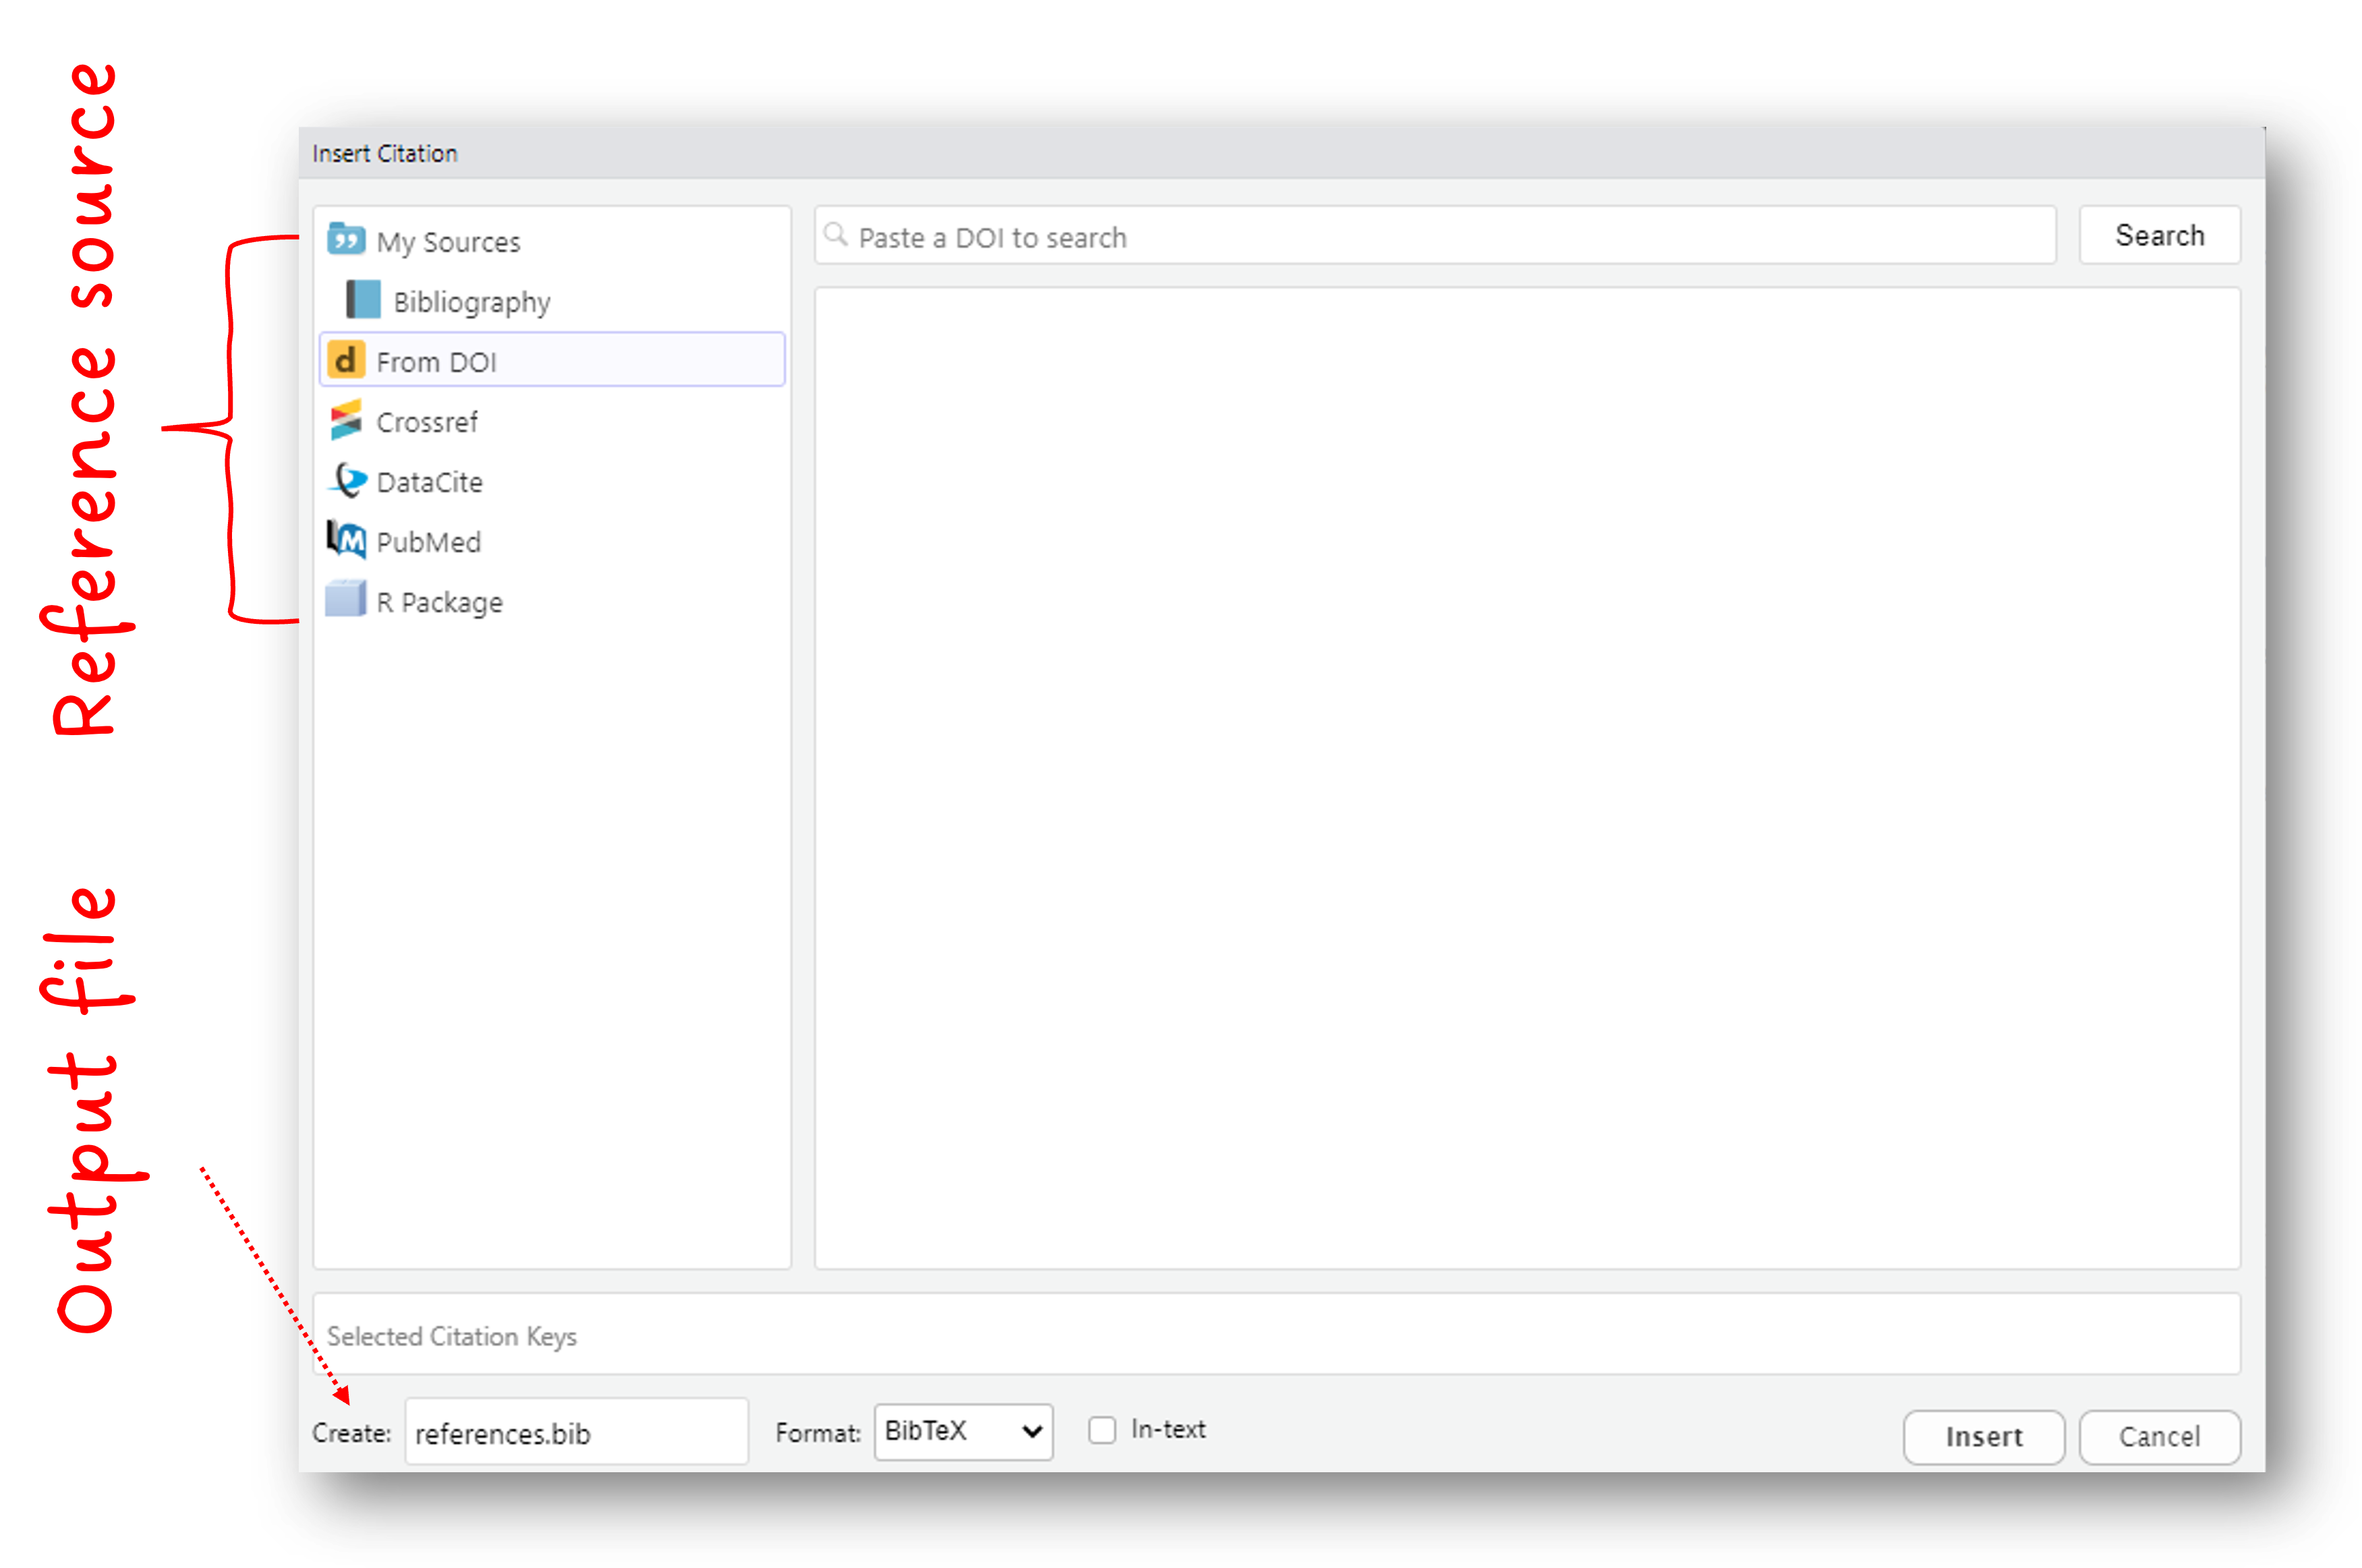
\includegraphics[width=5.15625in,height=\textheight]{images/referencing.png}
\end{center}

The reference you add will be saved to a \texttt{*.bib} that you can
access at the location where your \texttt{.qmd} file is stored. Once a
reference is added to your document, the YAML heading will display the
option \texttt{bibliography:\ references.bib} which is the source file
where your references are being managed.

\begin{tcolorbox}[enhanced jigsaw, left=2mm, toprule=.15mm, title={Task 3}, colbacktitle=quarto-callout-warning-color!10!white, toptitle=1mm, titlerule=0mm, breakable, opacityback=0, bottomrule=.15mm, coltitle=black, arc=.35mm, rightrule=.15mm, bottomtitle=1mm, colframe=quarto-callout-warning-color-frame, leftrule=.75mm, opacitybacktitle=0.6, colback=white]

\begin{enumerate}
\def\labelenumi{\arabic{enumi}.}
\tightlist
\item
  Copy and paste the following text under the \texttt{Introduction}
  section:
\end{enumerate}

\begin{Shaded}
\begin{Highlighting}[]
\NormalTok{There are hundreds of species of flowering plants, with one such genus known as the iris. Edgar Anderson procured measurements (in centimetres) from 150 different flowers from three different iris species [CITE]. The measurements are on the petal length and width, and sepal length and width from each flower. The three different iris species are the setosa, versicolor, and virginica. Here, we shall analyse the relationship between sepal width and sepal length and see whether the relationship, if any, is different across the three species of iris.}

\NormalTok{Section 2 consists of an exploratory analysis of the iris data and explores the potential relationship between sepal width and length, and whether there are any differences between the three species of the iris genus. Section 3 contains the results from fitting a multiple regression model to the data, as well as the assessment of the model assumptions. Concluding remarks are given in Section 4 .}
\end{Highlighting}
\end{Shaded}

\begin{enumerate}
\def\labelenumi{\arabic{enumi}.}
\setcounter{enumi}{1}
\tightlist
\item
  Then, change the species names (setosa, versicolor, and virginica) to
  \emph{italics} format and add a citation \texttt{{[}CITE{]}} for the
  iris data set using the following doi: \texttt{10.24432/C56C76} .
\item
  Lastly, change the text referring to to Section 2, 3 and 4 with
  clickable hyperlinks to each of these sections. Render
  
\includegraphics[width=0.21875in,height=0.17708in]{images/rstudio-render-button.png}
  your Quarto document and check the HTML output.
\end{enumerate}

see solution

The introduction section of your quarto document should look like this
if you go to the \texttt{source\ mode:}

\begin{Shaded}
\begin{Highlighting}[]
\NormalTok{{-}{-}{-}}
\NormalTok{title: "Data Analysis: Example Report"}
\NormalTok{number{-}sections: true}
\NormalTok{{-}{-}{-}}

\NormalTok{\# Introduction \{\#sec{-}intro\}}

\NormalTok{There are hundreds of species of flowering plants, with one such genus known as the iris. Edgar Anderson procured measurements (in centimetres) from 150 different flowers from three different iris species [@r.a.fisher1936] . The measurements are on the petal length and width, and sepal length and width from each flower. The three different iris species are the *setosa*, *versicolor*, and *virginica*. Here, we shall analyse the relationship between sepal width and sepal length and see whether the relationship, if any, is different across the three species of iris.}

\NormalTok{@sec{-}eda consists of an exploratory analysis of the iris data and explores the potential relationship between sepal width and length, and whether there are any differences between the three species of the iris genus. @sec{-}fda contains the results from fitting a multiple regression model to the data, as well as the assessment of the model assumptions. Concluding remarks are given in @sec{-}con .}
\end{Highlighting}
\end{Shaded}

\end{tcolorbox}

\section{Embedding R code}\label{embedding-r-code}

\subsection{Code chunks}\label{code-chunks}

Code chunks allow for R code to be embedded within a document. Not only
can the code be easily included within a document, the code can also be
evaluated. Hence, you can produce an entire report based on an analysis
that is contained within a single file instead of having separate files
containing your R code, plot images and comments.

R Code can be evaluated directly on the Quarto document or in the R
console (the latter would be similar to run your code from an R script).
To select where you want your code to be evaluated click on the setting
options

\includegraphics[width=0.19792in,height=\textheight]{images/settings.png}
(next to the Render button

\includegraphics[width=0.22917in,height=\textheight]{images/rstudio-render-button.png}
) and choose between \texttt{Chunk\ Output\ Inline} (default) if you
want your code to be evaluated within the Quarto document or
\texttt{Chunk\ Output\ in\ Console} to evaluate your code directly on
the R console. If you select the latter, the following options will be
added to the document preamble:

\begin{Shaded}
\begin{Highlighting}[]
\NormalTok{editor\_options}\SpecialCharTok{:} 
\NormalTok{  chunk\_output\_type}\SpecialCharTok{:}\NormalTok{ inline}
\end{Highlighting}
\end{Shaded}

To add an R Code Chunk you can simply click on the

\includegraphics[width=0.30208in,height=\textheight]{images/chunk.png}
symbol (or using keyboard shortcut \texttt{cmd+alt+i} or
\texttt{ctrl+alt+i} for windows users) on either \texttt{visual} or
\texttt{source} modes.

R code chunks are identified with~\texttt{\{r\}} with multiple
(optional) chunk options which we can access by typing
\texttt{\#\textbar{}}~at the beginning of the line.

\section{\texorpdfstring{\texttt{visual} mode view}{visual mode view}}

If you are on visual mode the R chunks will appear as follow:

\begin{center}
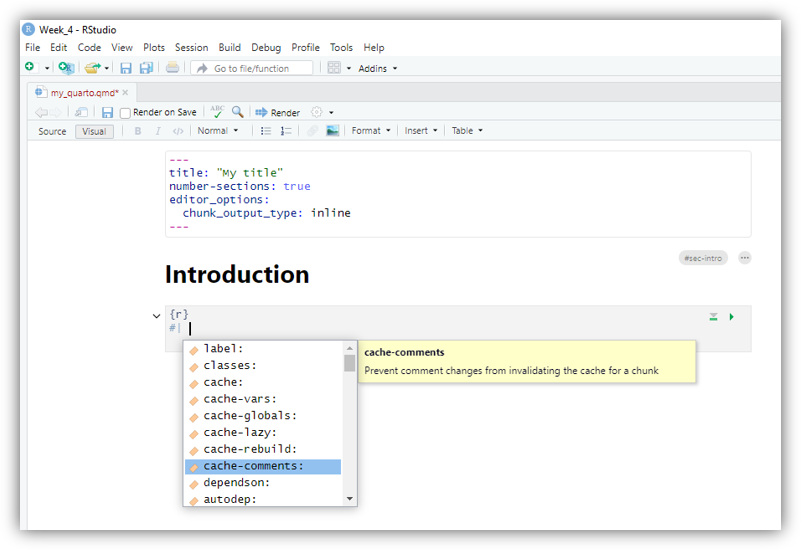
\includegraphics[width=5.05208in,height=\textheight]{images/quarto6.png}
\end{center}

\section{\texorpdfstring{\texttt{source} mode view}{source mode view}}

If you are in the source mode the R chunks will appear as follow:

\begin{Shaded}
\begin{Highlighting}[]
\InformationTok{\textasciigrave{}\textasciigrave{}\textasciigrave{}\{r\}}
\InformationTok{\#| }

\InformationTok{\textasciigrave{}\textasciigrave{}\textasciigrave{}}
\end{Highlighting}
\end{Shaded}

Some of the most common arguments you will use in your R Chunks are:

\begin{itemize}
\tightlist
\item
  \textbf{echo}: include the R code within the code chunk in the
  document (true/false);
\item
  \textbf{eval}: evaluate the R code within the code chunk (true/false);
\item
  \textbf{warning}: suppress warnings from R (true/false); and
\item
  \textbf{message}: suppress messages from R (true/false).
\end{itemize}

For example, let's say we wanted to select the \texttt{Sepal.Length},
\texttt{Sepal.Width} and \texttt{Species} variables from the
\texttt{iris} data set ( available by default from the \texttt{datasets}
library)to be used later, we can do that using the following code chunk:

\begin{Shaded}
\begin{Highlighting}[]
\NormalTok{\{r\}}
\CommentTok{\#| echo: false}
\FunctionTok{library}\NormalTok{(tidyverse)}

\NormalTok{iris\_subset }\OtherTok{\textless{}{-}}\NormalTok{ iris }\SpecialCharTok{\%\textgreater{}\%}
\NormalTok{   dplyr}\SpecialCharTok{::}\FunctionTok{select}\NormalTok{(Sepal.Width, Sepal.Length, Species)}
\end{Highlighting}
\end{Shaded}

Setting \texttt{echo:\ false} will tell the R to evaluate the code while
hiding the R chunk source code from the main document. In this example,
we will store the subsetted data set as the object \texttt{iris\_subset}
so that it can be used in chunks downstream. If you want to embed the
source code within the Quarto document then you would simply set
\texttt{echo:\ true}.

\begin{tcolorbox}[enhanced jigsaw, left=2mm, toprule=.15mm, title=\textcolor{quarto-callout-important-color}{\faExclamation}\hspace{0.5em}{Important}, colbacktitle=quarto-callout-important-color!10!white, toptitle=1mm, titlerule=0mm, breakable, opacityback=0, bottomrule=.15mm, coltitle=black, arc=.35mm, rightrule=.15mm, bottomtitle=1mm, colframe=quarto-callout-important-color-frame, leftrule=.75mm, opacitybacktitle=0.6, colback=white]

R chunk options are case sensitive! so \texttt{echo:\ TRUE} or
\texttt{echo:\ FALSE} won't work! You can use R Studio autocomplete
feature the see the available options by pressing the tab key.

\end{tcolorbox}

Note that by default, and unless otherwise specified, chunk codes in
Quarto will be set to \texttt{echo:\ true}. Alternatively, you can edit
the Quarto YAML preamble and change the global output options to show or
hide all R chunks. You can do this within the \texttt{execute} options
as follows (you can manually override this by changing the \texttt{echo}
option in each individual chunk) :

\begin{Shaded}
\begin{Highlighting}[]
\SpecialCharTok{{-}{-}{-}}
\NormalTok{title}\SpecialCharTok{:} \StringTok{"Data Analysis: Example Report"}
\NormalTok{number}\SpecialCharTok{{-}}\NormalTok{sections}\SpecialCharTok{:}\NormalTok{ true}
\NormalTok{execute}\SpecialCharTok{:}
\NormalTok{  echo}\SpecialCharTok{:}\NormalTok{ false}
\SpecialCharTok{{-}{-}{-}}
\end{Highlighting}
\end{Shaded}

\begin{tcolorbox}[enhanced jigsaw, left=2mm, toprule=.15mm, title=\textcolor{quarto-callout-important-color}{\faExclamation}\hspace{0.5em}{Important}, colbacktitle=quarto-callout-important-color!10!white, toptitle=1mm, titlerule=0mm, breakable, opacityback=0, bottomrule=.15mm, coltitle=black, arc=.35mm, rightrule=.15mm, bottomtitle=1mm, colframe=quarto-callout-important-color-frame, leftrule=.75mm, opacitybacktitle=0.6, colback=white]

You need to be very careful with the indentation if you decide to change
the global settings of Quarto preamble!

\end{tcolorbox}

Lets look at another example:

\begin{Shaded}
\begin{Highlighting}[]
\CommentTok{\#| message: false}
\CommentTok{\#| warning: false}
\FunctionTok{library}\NormalTok{(ggplot2)}
\end{Highlighting}
\end{Shaded}

In this case, we set \texttt{warning} and \texttt{message} to
\texttt{false} to indicate that we want to suppress any warnings or
messages (e.g., the ones that you usually get when loading R packages).
Another useful option is \texttt{eval.} If we set \texttt{eval:\ false}
then we indicate that we don't want the chunk output to be included in
the rendered document (this is useful for example if we just want to
show our R code without rendering its output). For example the following
chunk will only show the code for creating \texttt{ggplot} object
without actually evaluating it:

\begin{Shaded}
\begin{Highlighting}[]
\CommentTok{\#| eval: false}
\FunctionTok{ggplot}\NormalTok{(iris\_subset, }\FunctionTok{aes}\NormalTok{(}\AttributeTok{x =}\NormalTok{ Sepal.Length,}
                \AttributeTok{y =}\NormalTok{ Sepal.Width, }
                \AttributeTok{color =}\NormalTok{ Species)) }\SpecialCharTok{+}
  \FunctionTok{geom\_point}\NormalTok{()}
\end{Highlighting}
\end{Shaded}

\begin{tcolorbox}[enhanced jigsaw, left=2mm, toprule=.15mm, title=\textcolor{quarto-callout-note-color}{\faInfo}\hspace{0.5em}{Note}, colbacktitle=quarto-callout-note-color!10!white, toptitle=1mm, titlerule=0mm, breakable, opacityback=0, bottomrule=.15mm, coltitle=black, arc=.35mm, rightrule=.15mm, bottomtitle=1mm, colframe=quarto-callout-note-color-frame, leftrule=.75mm, opacitybacktitle=0.6, colback=white]

Note that we can still run the code in each individual chunk (even if we
set \texttt{eval:\ false}) by clicking the run chunk
bottom
\includegraphics[width=0.29167in,height=0.1875in]{images/run_chunk.png}.
The code will be evaluated in either your \texttt{.qmd} file or in the
console depending on the Chunk output settings (this mean that you can
test your code in R but its output won't be rendered in the final
document). \textbf{This means you don't need a separate R script to test
your code!}😁

\end{tcolorbox}

Additional arguments can be passed to code chunks other than those
displayed above. The most useful ones other than those relate to figure
sizing and positioning and are discussed in the upcoming sections.

\begin{tcolorbox}[enhanced jigsaw, left=2mm, toprule=.15mm, title={Task 4}, colbacktitle=quarto-callout-warning-color!10!white, toptitle=1mm, titlerule=0mm, breakable, opacityback=0, bottomrule=.15mm, coltitle=black, arc=.35mm, rightrule=.15mm, bottomtitle=1mm, colframe=quarto-callout-warning-color-frame, leftrule=.75mm, opacitybacktitle=0.6, colback=white]

\begin{enumerate}
\def\labelenumi{\arabic{enumi}.}
\tightlist
\item
  Add a new chunk at the beginning of your document that loads the
  following R packages:
\end{enumerate}

\begin{Shaded}
\begin{Highlighting}[]
\FunctionTok{library}\NormalTok{(ggplot2) }
\FunctionTok{library}\NormalTok{(tidyverse)}
\FunctionTok{library}\NormalTok{(kableExtra) }
\FunctionTok{library}\NormalTok{(performance) }
\end{Highlighting}
\end{Shaded}

Make sure that the source code and messages/warnings outputs from
loading these libraries are hidden from your rendered document.

\begin{enumerate}
\def\labelenumi{\arabic{enumi}.}
\setcounter{enumi}{1}
\tightlist
\item
  Then, add another chunk beneath the exploratory analysis section where
  you create a subset of the \texttt{iris} data set containing the
  variables \texttt{Sepal.Width}, \texttt{Sepal.Length} and
  \texttt{Species}. Make sure that the source code for this chunk is
  also hidden in the final document.
\end{enumerate}

Then, click the

\includegraphics[width=0.25in,height=0.20833in]{images/rstudio-render-button.png}\texttt{Render}
button and compile your Quarto document to make sure that your markdown
formatting produces the expected output in your HTML document.

See solution

The two chunks you have created should look as follows:

\begin{Shaded}
\begin{Highlighting}[]
\CommentTok{\#| echo: false}
\CommentTok{\#| warning: false }
\CommentTok{\#| message: false }

\FunctionTok{library}\NormalTok{(ggplot2) }
\FunctionTok{library}\NormalTok{(tidyverse)}
\FunctionTok{library}\NormalTok{(kableExtra) }
\FunctionTok{library}\NormalTok{(performance) }
\end{Highlighting}
\end{Shaded}

\begin{Shaded}
\begin{Highlighting}[]
\CommentTok{\#| echo: false}
\NormalTok{ iris\_subset }\OtherTok{\textless{}{-}}\NormalTok{ iris }\SpecialCharTok{\%\textgreater{}\%}
\NormalTok{   dplyr}\SpecialCharTok{::}\FunctionTok{select}\NormalTok{(Sepal.Width, Sepal.Length, Species) }
\end{Highlighting}
\end{Shaded}

\end{tcolorbox}

\subsection{Inline code}\label{inline-code}

R code can be included within text by enclosing the code with
\texttt{\textasciigrave{}r\ \textasciigrave{}}. This allows for
expressions to be evaluated by R and not be hardwired by the user. For
example, if you wanted to convey the number of observations within
\texttt{iris\_subset} then we can enclose \texttt{nrow(iris\_subset)}
within \texttt{\textasciigrave{}r\ \textasciigrave{}} to obtain the
number of observations, rather than hardwiring 150 into the text. This
can help to prevent potential human error when presenting information.
It can also help with consistency and ease-of-use, since
\texttt{n\ =\ nrow(iris\_subset)} could be stored as an R object and
referred to whenever necessary within the text using inline R code.

\section{Tables}\label{tables}

There are several ways to produce tables in Quarto . Here, a couple of
different approaches will be presented. The first approach uses the
\texttt{kable()} function from the \texttt{kableExtra} package and
essentially receives a data frame as input and then puts a wrapper
around the tables produced in R in order to make them more visually
appealing within the Quarto document. Here we will just cover the
basics, but if you want to learn more about creating eye-catching tables
with \texttt{kableExtra} visit
\href{https://bookdown.org/yihui/rmarkdown-cookbook/kableextra.html}{here}.

Let's say we wanted to create a table of the mean and std. dev of the
sepal Length and width for each species in the \texttt{iris\_subset}
data. We can create the table using the \texttt{kable()} function as
follows:

\begin{Shaded}
\begin{Highlighting}[]
\NormalTok{iris\_summary }\OtherTok{\textless{}{-}}\NormalTok{ iris\_subset }\SpecialCharTok{\%\textgreater{}\%}
   \FunctionTok{summarise}\NormalTok{(}\StringTok{\textquotesingle{}Sepal.Width.Mean\textquotesingle{}} \OtherTok{=} \FunctionTok{mean}\NormalTok{(Sepal.Width),}
             \StringTok{\textquotesingle{}Sepal.Width.sd\textquotesingle{}} \OtherTok{=} \FunctionTok{sd}\NormalTok{(Sepal.Width),}
             \StringTok{\textquotesingle{}Sepal.Length.Mean\textquotesingle{}} \OtherTok{=} \FunctionTok{mean}\NormalTok{(Sepal.Length),}
             \StringTok{\textquotesingle{}Sepal.Length.sd\textquotesingle{}} \OtherTok{=} \FunctionTok{sd}\NormalTok{(Sepal.Length),}
             \AttributeTok{.by =}\NormalTok{ Species) }
\NormalTok{iris\_summary }\SpecialCharTok{\%\textgreater{}\%}
  \FunctionTok{kable}\NormalTok{() }
\end{Highlighting}
\end{Shaded}

\begin{longtable}[]{@{}
  >{\raggedright\arraybackslash}p{(\columnwidth - 8\tabcolsep) * \real{0.1429}}
  >{\raggedleft\arraybackslash}p{(\columnwidth - 8\tabcolsep) * \real{0.2208}}
  >{\raggedleft\arraybackslash}p{(\columnwidth - 8\tabcolsep) * \real{0.1948}}
  >{\raggedleft\arraybackslash}p{(\columnwidth - 8\tabcolsep) * \real{0.2338}}
  >{\raggedleft\arraybackslash}p{(\columnwidth - 8\tabcolsep) * \real{0.2078}}@{}}
\toprule\noalign{}
\begin{minipage}[b]{\linewidth}\raggedright
Species
\end{minipage} & \begin{minipage}[b]{\linewidth}\raggedleft
Sepal.Width.Mean
\end{minipage} & \begin{minipage}[b]{\linewidth}\raggedleft
Sepal.Width.sd
\end{minipage} & \begin{minipage}[b]{\linewidth}\raggedleft
Sepal.Length.Mean
\end{minipage} & \begin{minipage}[b]{\linewidth}\raggedleft
Sepal.Length.sd
\end{minipage} \\
\midrule\noalign{}
\endhead
\bottomrule\noalign{}
\endlastfoot
setosa & 3.428 & 0.3790644 & 5.006 & 0.3524897 \\
versicolor & 2.770 & 0.3137983 & 5.936 & 0.5161711 \\
virginica & 2.974 & 0.3224966 & 6.588 & 0.6358796 \\
\end{longtable}

Lets customize this table a bit by (1) adding a table caption and a
cross-referencing number (2) modifying the labels of the columns and (3)
rounding the number of decimal places to two:

\begin{Shaded}
\begin{Highlighting}[]
\InformationTok{\textasciigrave{}\textasciigrave{}\textasciigrave{}\{r\}}
\InformationTok{\#| label: tbl{-}iris}
\InformationTok{\#| tbl{-}cap:  Mean and standard deviation (sd) sepal width and length by species of iris.}

\InformationTok{iris\_summary \%\textgreater{}\%}
\InformationTok{  kable(col.names = c("Species",}
\InformationTok{                      "Sepal mean width (cm)",}
\InformationTok{                      "Sepal width std.dev (cm)",}
\InformationTok{                      "Sepal mean length (cm)",}
\InformationTok{                      "Sepal width std.dev (cm)"),}
\InformationTok{        digits = 2) }
\InformationTok{\textasciigrave{}\textasciigrave{}\textasciigrave{}}
\end{Highlighting}
\end{Shaded}

\begin{longtable}[]{@{}
  >{\raggedright\arraybackslash}p{(\columnwidth - 8\tabcolsep) * \real{0.1038}}
  >{\raggedleft\arraybackslash}p{(\columnwidth - 8\tabcolsep) * \real{0.2075}}
  >{\raggedleft\arraybackslash}p{(\columnwidth - 8\tabcolsep) * \real{0.2358}}
  >{\raggedleft\arraybackslash}p{(\columnwidth - 8\tabcolsep) * \real{0.2170}}
  >{\raggedleft\arraybackslash}p{(\columnwidth - 8\tabcolsep) * \real{0.2358}}@{}}

\caption{\label{tbl-iris}Mean and standard deviation (sd) sepal width
and length by species of iris.}

\tabularnewline

\toprule\noalign{}
\begin{minipage}[b]{\linewidth}\raggedright
Species
\end{minipage} & \begin{minipage}[b]{\linewidth}\raggedleft
Sepal mean width (cm)
\end{minipage} & \begin{minipage}[b]{\linewidth}\raggedleft
Sepal width std.dev (cm)
\end{minipage} & \begin{minipage}[b]{\linewidth}\raggedleft
Sepal mean length (cm)
\end{minipage} & \begin{minipage}[b]{\linewidth}\raggedleft
Sepal width std.dev (cm)
\end{minipage} \\
\midrule\noalign{}
\endhead
\bottomrule\noalign{}
\endlastfoot
setosa & 3.43 & 0.38 & 5.01 & 0.35 \\
versicolor & 2.77 & 0.31 & 5.94 & 0.52 \\
virginica & 2.97 & 0.32 & 6.59 & 0.64 \\

\end{longtable}

The first thing we've done is to add a table label using
\texttt{label:\ tbl-iris} in the chunk options.This will allow us to add
cross-reference in the text (remember to use the \texttt{tbl-}~prefix to
make them cross-referenceable). For example we can write
\texttt{@tbl-iris} in our document to reference and create an hyperlink
directed to the Table~\ref{tbl-iris} (you can also use the tool bar
\texttt{Insert▾➠\ Cross\ Reference} to do this). Then, the chunk option
\texttt{tbl-cap:} allow us to add caption to the table. To make the
table more appealing we can make the table more appealing by setting the
number of decimals to 2 by setting \texttt{digits\ =\ 2}. Lastly, we
modify the original column names via the \texttt{col.names} argument.

\begin{tcolorbox}[enhanced jigsaw, left=2mm, toprule=.15mm, title={Task 5}, colbacktitle=quarto-callout-warning-color!10!white, toptitle=1mm, titlerule=0mm, breakable, opacityback=0, bottomrule=.15mm, coltitle=black, arc=.35mm, rightrule=.15mm, bottomtitle=1mm, colframe=quarto-callout-warning-color-frame, leftrule=.75mm, opacitybacktitle=0.6, colback=white]

Add two separate chunks in your exploratory analysis that produce the
following tables:

\begin{enumerate}
\def\labelenumi{\arabic{enumi}.}
\item
  A table displaying the mean, median and standard deviation for sepal
  width and length for each of the three different species of iris.
\item
  A table displaying the Pearson correlation between sepal width and
  length by species.
\end{enumerate}

Round each value to 2 decimals and use appropriate column headings for
each table. Then add a sensible table caption and a cross-referencing
number. Comment on this output in the main body of your document while
using clickable hyperlinks whenever referencing each table.

Before you render your document make sure that the source code for these
chunks is hidden.

Take hint

Use the \texttt{summarise} function in conjunction with the
\texttt{cor()} function to compute the Pearson correlation between sepal
length and width for each species.

See solution

Your chunks should look something like this:

\begin{Shaded}
\begin{Highlighting}[]
\CommentTok{\#| echo: false}
\CommentTok{\#| label: tbl{-}summary}
\CommentTok{\#| tbl{-}cap:  Mean, median and standard deviation (sd) sepal width and length by species of iris.}

\NormalTok{iris\_summary }\OtherTok{\textless{}{-}}\NormalTok{ iris\_subset }\SpecialCharTok{\%\textgreater{}\%}
   \FunctionTok{summarise}\NormalTok{(}\StringTok{\textquotesingle{}Sepal.Width.Mean\textquotesingle{}} \OtherTok{=} \FunctionTok{mean}\NormalTok{(Sepal.Width),}
             \StringTok{\textquotesingle{}Sepal.Width.Medain\textquotesingle{}} \OtherTok{=} \FunctionTok{median}\NormalTok{(Sepal.Width),}
             \StringTok{\textquotesingle{}Sepal.Width.sd\textquotesingle{}} \OtherTok{=} \FunctionTok{sd}\NormalTok{(Sepal.Width),}
             \StringTok{\textquotesingle{}Sepal.Length.Mean\textquotesingle{}} \OtherTok{=} \FunctionTok{mean}\NormalTok{(Sepal.Length),}
             \StringTok{\textquotesingle{}Sepal.Length.Medain\textquotesingle{}} \OtherTok{=} \FunctionTok{median}\NormalTok{(Sepal.Length),}
             \StringTok{\textquotesingle{}Sepal.Length.sd\textquotesingle{}} \OtherTok{=} \FunctionTok{sd}\NormalTok{(Sepal.Length),}
             \AttributeTok{.by =}\NormalTok{ Species) }

\NormalTok{iris\_summary }\SpecialCharTok{\%\textgreater{}\%}
  \FunctionTok{kable}\NormalTok{(}\AttributeTok{col.names =} \FunctionTok{c}\NormalTok{(}\StringTok{"Species"}\NormalTok{,}
                      \StringTok{"Sepal mean width (cm)"}\NormalTok{,}
                      \StringTok{"Sepalmedian width (cm)"}\NormalTok{,}
                      \StringTok{"Sepal width std.dev (cm)"}\NormalTok{,}
                      \StringTok{"Sepal mean length (cm)"}\NormalTok{,}
                      \StringTok{"Sepal median length (cm)"}\NormalTok{,}
                      \StringTok{"Sepal width std.dev (cm)"}\NormalTok{),}
        \AttributeTok{digits =} \DecValTok{2}\NormalTok{)}
\end{Highlighting}
\end{Shaded}

\begin{Shaded}
\begin{Highlighting}[]
\CommentTok{\#| echo: false}
\CommentTok{\#| label: tbl{-}cor}
\CommentTok{\#| tbl{-}cap: Correlation between sepal width and length by species.}

\NormalTok{Cors }\OtherTok{\textless{}{-}}\NormalTok{ iris\_subset }\SpecialCharTok{\%\textgreater{}\%}
        \FunctionTok{summarise}\NormalTok{(}\StringTok{\textquotesingle{}Correlation\textquotesingle{}} \OtherTok{=} \FunctionTok{cor}\NormalTok{(Sepal.Width, Sepal.Length),}
                  \AttributeTok{.by =}\NormalTok{ Species)}
\NormalTok{Cors }\SpecialCharTok{\%\textgreater{}\%}
  \FunctionTok{kable}\NormalTok{(}\AttributeTok{digits=}\DecValTok{2}\NormalTok{)}
\end{Highlighting}
\end{Shaded}

Then, \texttt{@tbl-summary} and \texttt{@tbl-cor} should be used in the
text to reference the corresponding table.

\end{tcolorbox}

\subsection{Tables `by hand'}\label{tables-by-hand}

Tables can also be produced `by hand' in Quarto. Here is an example of
how we can recreate the table above corresponding to the first 5 rows of
the \texttt{iris} data.

\section{\texorpdfstring{\texttt{visual} mode view}{visual mode view}}

On visual mode, this table can be created by clicking on the
\texttt{Table} option in the toolbar (next to \texttt{Insert▾} while
using the \texttt{visual} mode) and selecting the number of rows and
columns. Here you can also add a caption to the table.

\begin{center}
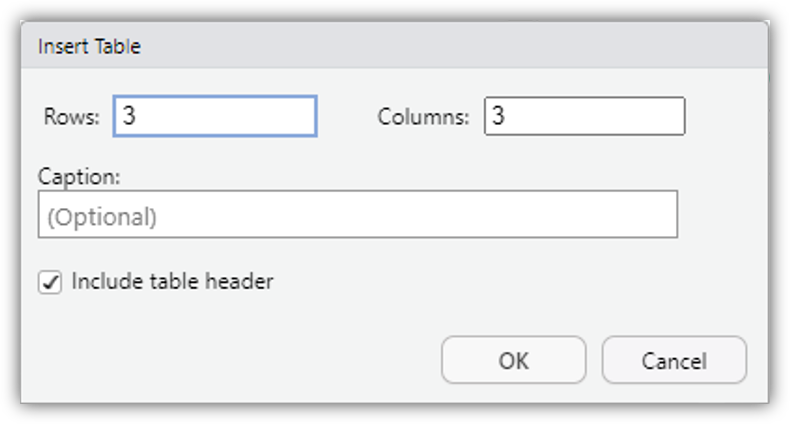
\includegraphics[width=4.53125in,height=\textheight]{images/quarto7.png}
\end{center}

We can manually fill each entry to produce the following table:

\begin{longtable}[]{@{}ccccr@{}}
\caption{The fist 5 rows of the iris data.}\tabularnewline
\toprule\noalign{}
Sepal Length & Sepal Width & Petal Length & Petal Width & Species \\
\midrule\noalign{}
\endfirsthead
\toprule\noalign{}
Sepal Length & Sepal Width & Petal Length & Petal Width & Species \\
\midrule\noalign{}
\endhead
\bottomrule\noalign{}
\endlastfoot
5.1 & 3.5 & 1.4 & 0.2 & setosa \\
4.9 & 3.0 & 1.4 & 0.2 & setosa \\
4.7 & 3.2 & 1.3 & 0.2 & setosa \\
4.6 & 3.1 & 1.5 & 0.2 & setosa \\
5.0 & 3.6 & 1.4 & 0.2 & setosa \\
\end{longtable}

\section{\texorpdfstring{\texttt{source} mode view}{source mode view}}

On \texttt{source} mode, the raw markdown code that produces this table
is the following:

\begin{verbatim}
| Sepal Length | Sepal Width | Petal Length | Petal Width | Species |
|:------------:|:-----------:|:------------:|:-----------:|--------:|
|     5.1      |     3.5     |     1.4      |     0.2     |  setosa |
|     4.9      |     3.0     |     1.4      |     0.2     |  setosa |
|     4.7      |     3.2     |     1.3      |     0.2     |  setosa |
|     4.6      |     3.1     |     1.5      |     0.2     |  setosa |
|     5.0      |     3.6     |     1.4      |     0.2     |  setosa |
: The fist 5 rows of the iris data. {#tbl-iris}
\end{verbatim}

In here, the vertical separators \texttt{\textbar{}} are used between
columns, while \texttt{-\/-\/-} is placed below table/column headings.
Alignment of the columns is done using colons, that is, for left
alignment put \texttt{:-\/-\/-}, for right alignment put
\texttt{-\/-\/-:}, and for centred alignment put \texttt{:-\/-\/-:}. For
these sorts of tables, you can add a caption below the table and then
include a \texttt{\#tbl-\ label} in braces at the end of the caption for
cross-referencing.

For example, the table above corresponding to the first 5 rows of the
\texttt{iris} data can be produced by hand by clicking on the
\texttt{Table} option in the toolbar (next to \texttt{Insert▾} while
using the \texttt{visual} mode) and selecting the number of rows and
columns.

\begin{tcolorbox}[enhanced jigsaw, left=2mm, toprule=.15mm, title=\textcolor{quarto-callout-note-color}{\faInfo}\hspace{0.5em}{Note}, colbacktitle=quarto-callout-note-color!10!white, toptitle=1mm, titlerule=0mm, breakable, opacityback=0, bottomrule=.15mm, coltitle=black, arc=.35mm, rightrule=.15mm, bottomtitle=1mm, colframe=quarto-callout-note-color-frame, leftrule=.75mm, opacitybacktitle=0.6, colback=white]

You can read more about authoring Quarto tables
\href{https://quarto.org/docs/authoring/tables.html}{here}.

\end{tcolorbox}

\subsection{\texorpdfstring{\textbf{Summary of Regression Models as HTML
Tables}}{Summary of Regression Models as HTML Tables}}\label{summary-of-regression-models-as-html-tables}

In this section we briefly introduce the package \texttt{sjPlot} to
create HTML-tables that will be displayed nicely in your Quarto
document. We will focus on the \texttt{tab\_model()} function, which
receives as argument a single or multiple models fitted with the
\texttt{lm} or \texttt{glm} engine (other models, like hurdle- or
zero-inflated models, also work with this function).

\begin{tcolorbox}[enhanced jigsaw, left=2mm, toprule=.15mm, title=\textcolor{quarto-callout-important-color}{\faExclamation}\hspace{0.5em}{Important}, colbacktitle=quarto-callout-important-color!10!white, toptitle=1mm, titlerule=0mm, breakable, opacityback=0, bottomrule=.15mm, coltitle=black, arc=.35mm, rightrule=.15mm, bottomtitle=1mm, colframe=quarto-callout-important-color-frame, leftrule=.75mm, opacitybacktitle=0.6, colback=white]

HTML is the only output-format, you can't (directly) create a LaTeX or
PDF output
from~\href{https://strengejacke.github.io/sjPlot/reference/tab_model.html}{\texttt{tab\_model()}}~and
related table-functions.~

\end{tcolorbox}

For example, say we want to create a nice html table of a linear model
fitted to the \texttt{iris\_subset} data set:

\begin{Shaded}
\begin{Highlighting}[]
\FunctionTok{library}\NormalTok{(sjPlot)}
\NormalTok{int.model }\OtherTok{\textless{}{-}} \FunctionTok{lm}\NormalTok{(Sepal.Width }\SpecialCharTok{\textasciitilde{}}\NormalTok{ Sepal.Length }\SpecialCharTok{*}\NormalTok{ Species, }\AttributeTok{data =}\NormalTok{ iris\_subset)}
\end{Highlighting}
\end{Shaded}

Then we can simply add the following chunk to display the
Table~\ref{tbl-lm_iris} below:

\begin{Shaded}
\begin{Highlighting}[]
\CommentTok{\#| tbl{-}cap: "Summaries of the linear model fitted to the iries  data set."}
\CommentTok{\#| label: tbl{-}lm\_iris}
\FunctionTok{tab\_model}\NormalTok{(int.model)}
\end{Highlighting}
\end{Shaded}

\begin{longtable}[]{@{}
  >{\centering\arraybackslash}p{(\columnwidth - 6\tabcolsep) * \real{0.2500}}
  >{\centering\arraybackslash}p{(\columnwidth - 6\tabcolsep) * \real{0.2500}}
  >{\centering\arraybackslash}p{(\columnwidth - 6\tabcolsep) * \real{0.2500}}
  >{\centering\arraybackslash}p{(\columnwidth - 6\tabcolsep) * \real{0.2500}}@{}}

\caption{\label{tbl-lm_iris}Summaries of the linear model fitted to the
iries data set.}

\tabularnewline

\toprule\noalign{}
\endhead
\bottomrule\noalign{}
\endlastfoot
~ &
\multicolumn{3}{>{\centering\arraybackslash}p{(\columnwidth - 6\tabcolsep) * \real{0.7500} + 4\tabcolsep}@{}}{%
Sepal Width} \\
Predictors & Estimates & CI & p \\
(Intercept) & -0.57 & -1.66~--~0.53 & 0.306 \\
Sepal Length & 0.80 & 0.58~--~1.02 & \textbf{\textless0.001} \\
Species {[}versicolor{]} & 1.44 & 0.03~--~2.85 & \textbf{0.045} \\
Species {[}virginica{]} & 2.02 & 0.66~--~3.37 & \textbf{0.004} \\
\begin{minipage}[t]{\linewidth}\raggedright
Sepal Length × Species\\
{[}versicolor{]}\strut
\end{minipage} & -0.48 & -0.74~--~-0.21 & \textbf{\textless0.001} \\
\begin{minipage}[t]{\linewidth}\raggedright
Sepal Length × Species\\
{[}virginica{]}\strut
\end{minipage} & -0.57 & -0.82~--~-0.32 & \textbf{\textless0.001} \\
Observations &
\multicolumn{3}{>{\raggedright\arraybackslash}p{(\columnwidth - 6\tabcolsep) * \real{0.7500} + 4\tabcolsep}@{}}{%
150} \\
R\textsuperscript{2} / R\textsuperscript{2} adjusted &
\multicolumn{3}{>{\raggedright\arraybackslash}p{(\columnwidth - 6\tabcolsep) * \real{0.7500} + 4\tabcolsep}@{}}{%
0.623 / 0.610} \\

\end{longtable}

\href{https://strengejacke.github.io/sjPlot/reference/tab_model.html}{\texttt{tab\_model()}}
has some argument that allow to show or hide specific columns from the
output:

\begin{itemize}
\item
  \texttt{show.ci} to show/hide the column with confidence intervals.
\item
  \texttt{show.se} to show/hide the column with standard errors.
\item
  \texttt{show.p} to show/hide the column with p-values.
\item
  \texttt{show.r2} to show/hide \(R^2\) values.
\item
  \texttt{show.obs} to show/hide the number of observation.
\end{itemize}

Other useful arguments are \texttt{collapse.ci}~and~\texttt{collapse.se}
which collapse the columns for confidence intervals and standard errors
(i.e., one column together with the estimates). You can use the
\texttt{pred.labels} argument to change the names of the coefficients in
the \emph{Predictors} column (note that the length of
\texttt{pred.labels} must exactly match the amount of predictors in the
\emph{Predictor} column).

Lastly, \texttt{tab\_model()}~can also be used to print multiple models
at once, which are then printed side-by-side, e.g.,
\texttt{tab\_model(model\_1,\ model\_2)}. You ca use the
\texttt{dv.labels} to change the names of the model columns, this way
you can give sensible name to each model.

\begin{tcolorbox}[enhanced jigsaw, left=2mm, toprule=.15mm, title=\textcolor{quarto-callout-note-color}{\faInfo}\hspace{0.5em}{Note}, colbacktitle=quarto-callout-note-color!10!white, toptitle=1mm, titlerule=0mm, breakable, opacityback=0, bottomrule=.15mm, coltitle=black, arc=.35mm, rightrule=.15mm, bottomtitle=1mm, colframe=quarto-callout-note-color-frame, leftrule=.75mm, opacitybacktitle=0.6, colback=white]

You can read more about \texttt{sjPlot} html regression model tables
\href{https://strengejacke.github.io/sjPlot/articles/tab_model_estimates.html}{here}.

\end{tcolorbox}

\section{Figures}\label{figures}

\subsection{Embedding external images}\label{embedding-external-images}

Including plots and figures within a Quarto document is straightforward.
To include an external figure you can use the \texttt{visual} mode tool
bar and click on \texttt{Insert▾➠\ Figure/Image...} and then browse to
the path where you image is, or alternatively write the \emph{url} from
which the image should be obtained. The pop-up windows allows you also
to write a caption and also to modify the image alignment with respect
the main text.

\begin{center}
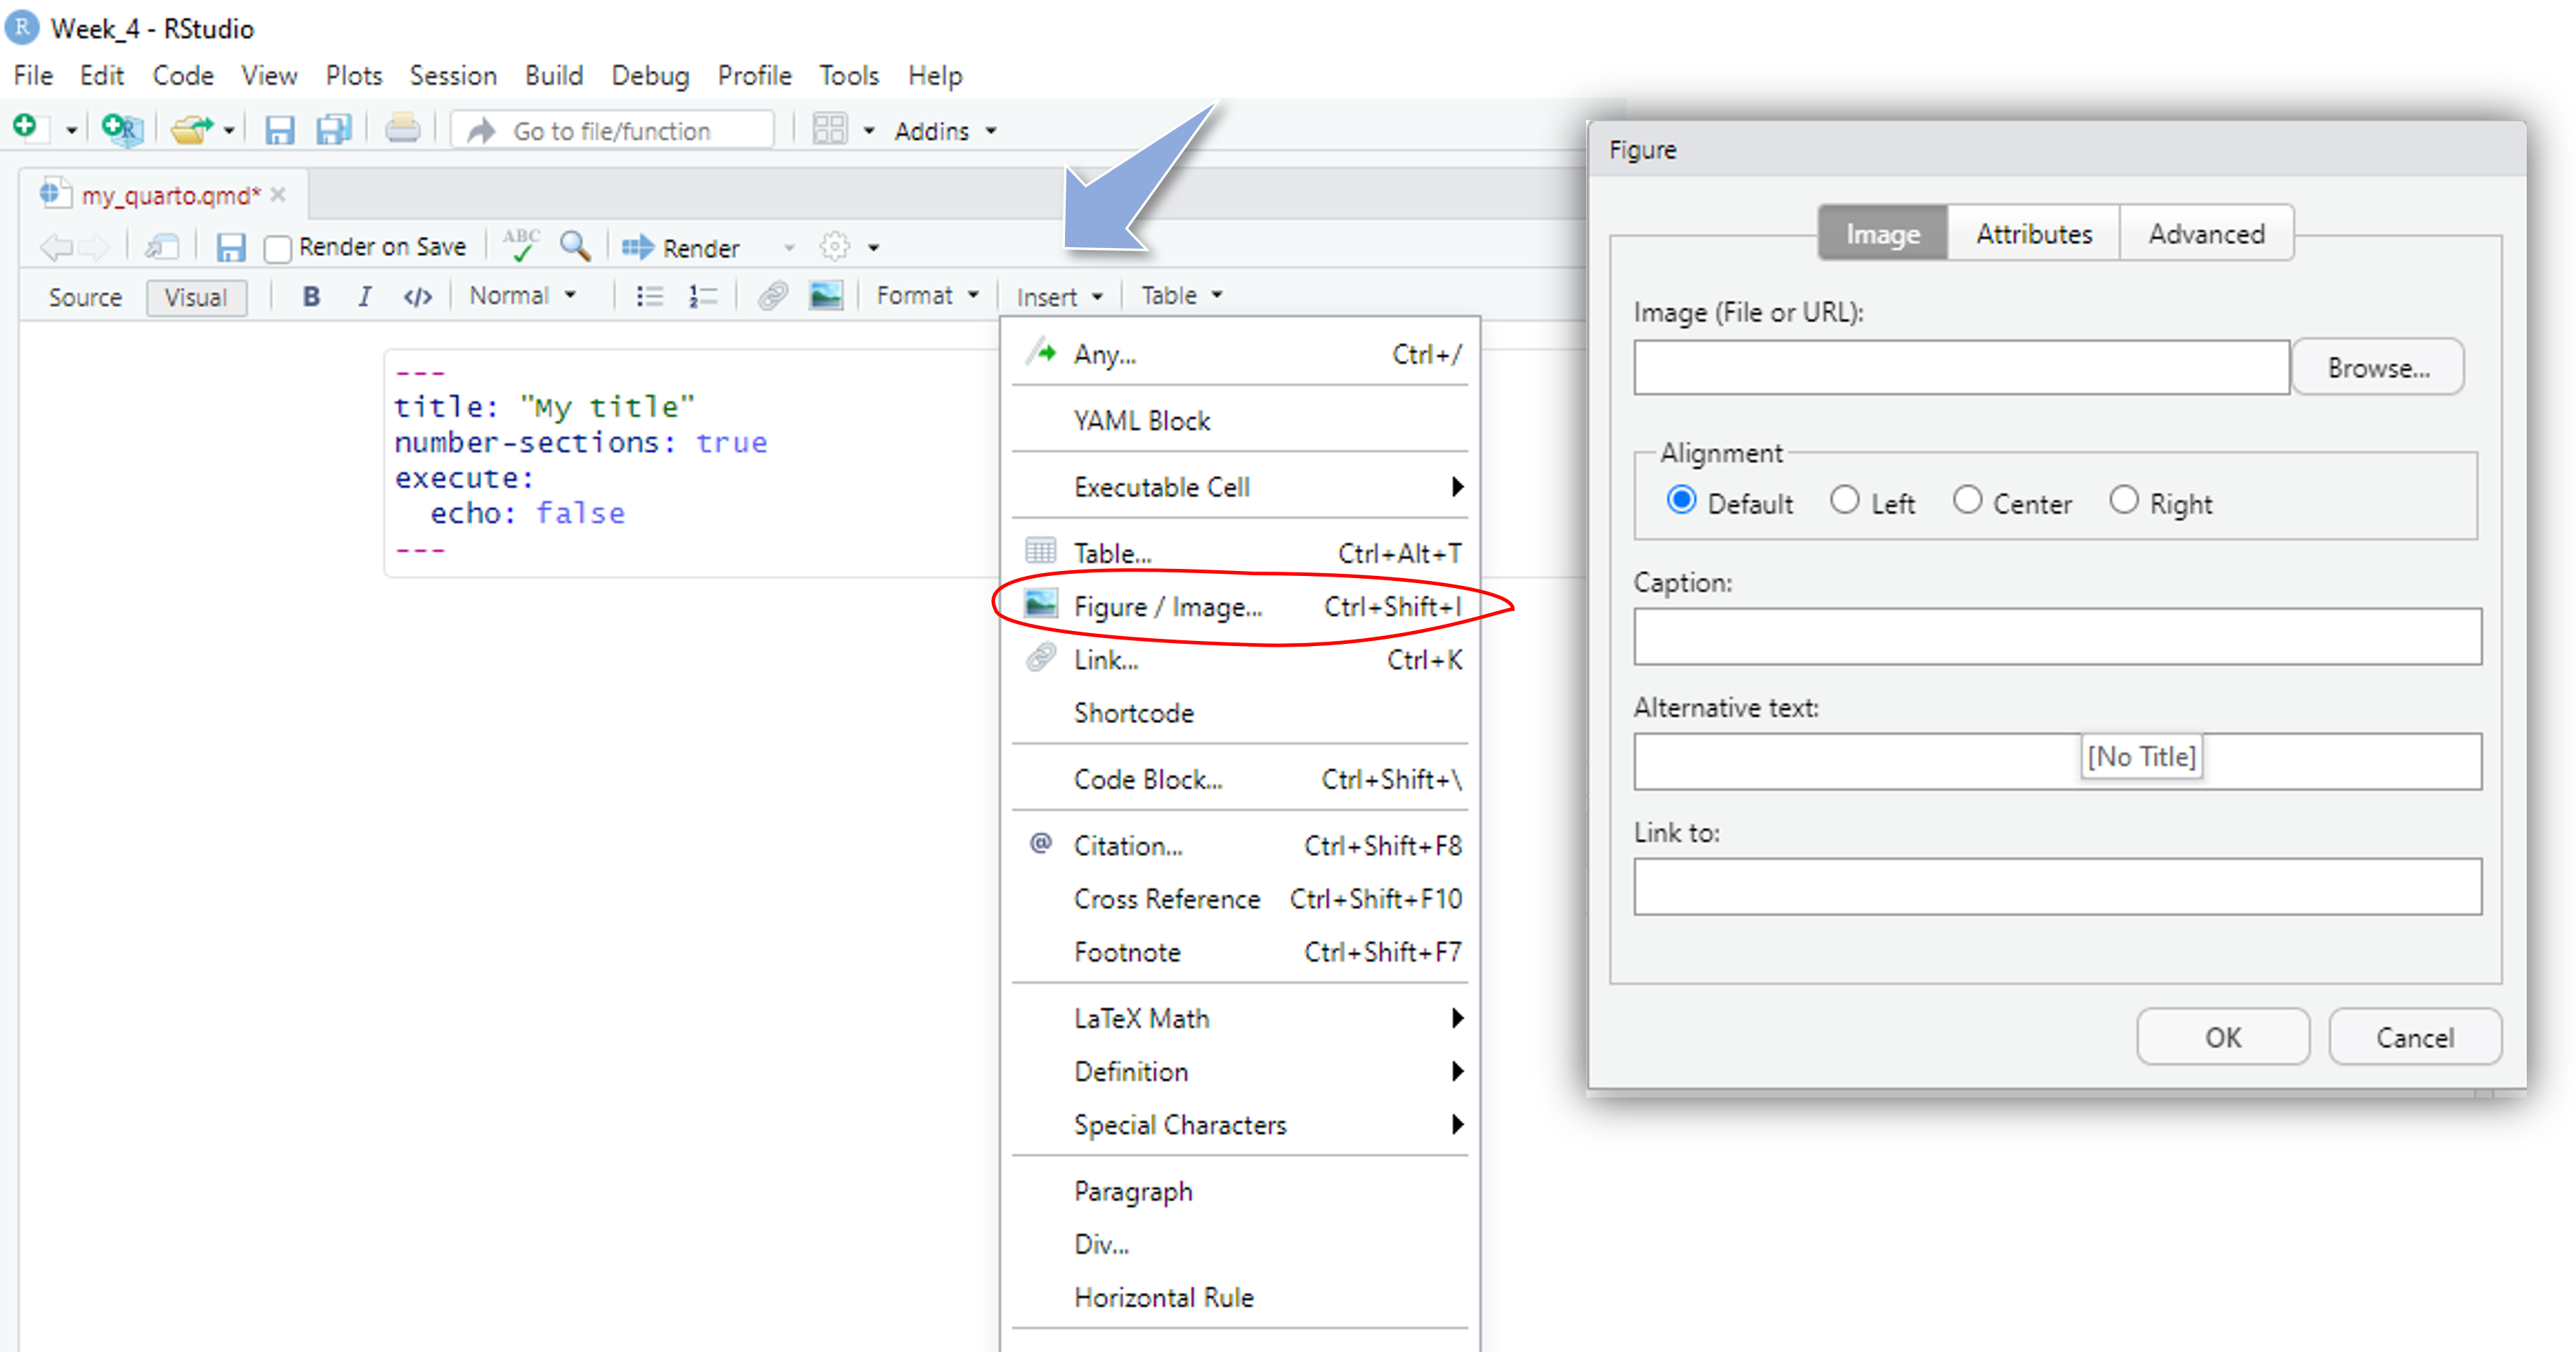
\includegraphics{images/quarto8.png}
\end{center}

If you want to add cross-referencing you can add the \texttt{fig-}
prefix in the attributes tab of the pop-up windows:

\begin{center}
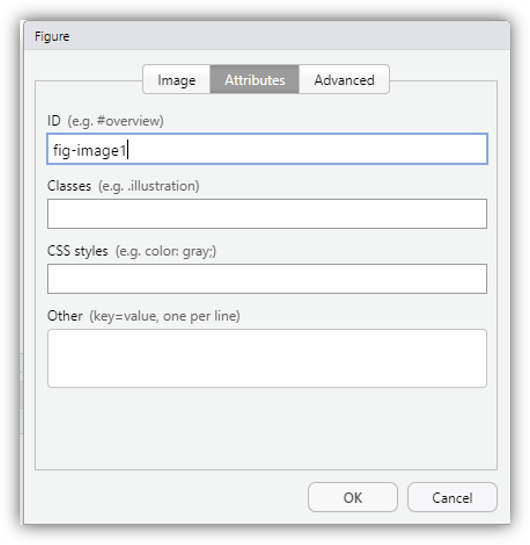
\includegraphics[width=3.94792in,height=\textheight]{images/quarto9.png}
\end{center}

The source code would then look something like:

\begin{Shaded}
\begin{Highlighting}[]
\SpecialCharTok{!}\NormalTok{[](images}\SpecialCharTok{/}\NormalTok{myimage.png)\{}\CommentTok{\#fig{-}image1\}}
\end{Highlighting}
\end{Shaded}

\subsection{Embedding R generated
figures}\label{embedding-r-generated-figures}

Very often we would like to use the R plots generated from your analysis
instead of using external figures. To achieve this, the R code for the
plot is simply included within a code chunk including additional
arguments for plot size and positioning. For example, to include the
scatterplot of sepal width and length by species:

\section{R ggplot}

\begin{figure}

\centering{

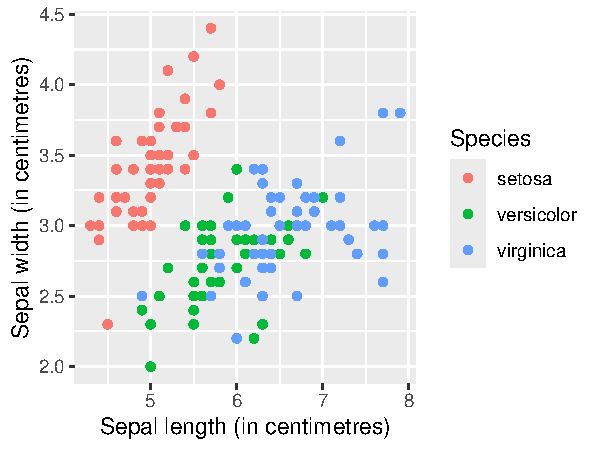
\includegraphics{notes_files/figure-pdf/fig-scatterplot1-1.pdf}

}

\caption{\label{fig-scatterplot1}Relationship between sepal width and
sepal length by species.}

\end{figure}%

\section{R chunk code}

\begin{Shaded}
\begin{Highlighting}[]
\CommentTok{\#| label: fig{-}scatterplot1}
\CommentTok{\#| fig{-}cap: Relationship between sepal width and sepal length by species.}
\CommentTok{\#| fig{-}width: 4}
\CommentTok{\#| fig{-}height: 3}
\CommentTok{\#| fig{-}align: center}
\CommentTok{\#| message: false}


\FunctionTok{ggplot}\NormalTok{(iris\_subset, }\FunctionTok{aes}\NormalTok{(}\AttributeTok{x =}\NormalTok{ Sepal.Length, }\AttributeTok{y =}\NormalTok{ Sepal.Width, }\AttributeTok{color =}\NormalTok{ Species)) }\SpecialCharTok{+}
  \FunctionTok{geom\_point}\NormalTok{() }\SpecialCharTok{+}
  \FunctionTok{labs}\NormalTok{(}\AttributeTok{x =} \StringTok{"Sepal length (in centimetres)"}\NormalTok{, }\AttributeTok{y =} \StringTok{"Sepal width (in centimetres)"}\NormalTok{, }\AttributeTok{color =} \StringTok{"Species"}\NormalTok{) }
\end{Highlighting}
\end{Shaded}

Here, we set the chunk label to include the \texttt{fig-} prefix so we
can cross-reference using the @ prefix. For example
\texttt{@fig-scatterplot1} will create a hyperlink to
Figure~\ref{fig-scatterplot1}. Then we added a figure caption using the
\texttt{fig-cap} option. For size and positioning of the figure we can
include:

\begin{itemize}
\tightlist
\item
  \texttt{fig.width}: an integer value denoting the width of the figure;
\item
  \texttt{fig.height}: an integer value denoting the height of the
  figure;
\item
  \texttt{fig.align}: the alignment of the figure within the body of the
  document
\end{itemize}

\begin{tcolorbox}[enhanced jigsaw, left=2mm, toprule=.15mm, title={Question}, colbacktitle=quarto-callout-tip-color!10!white, toptitle=1mm, titlerule=0mm, breakable, opacityback=0, bottomrule=.15mm, coltitle=black, arc=.35mm, rightrule=.15mm, bottomtitle=1mm, colframe=quarto-callout-tip-color-frame, leftrule=.75mm, opacitybacktitle=0.6, colback=white]

What other argument would you need to include if you wish to show the
chunk plot output only?

\begin{itemize}
\tightlist
\item
  \begin{enumerate}
  \def\labelenumi{(\Alph{enumi})}
  \tightlist
  \item
    eval: false\\
  \end{enumerate}
\item
  \begin{enumerate}
  \def\labelenumi{(\Alph{enumi})}
  \setcounter{enumi}{1}
  \tightlist
  \item
    echo: true\\
  \end{enumerate}
\item
  \begin{enumerate}
  \def\labelenumi{(\Alph{enumi})}
  \setcounter{enumi}{2}
  \tightlist
  \item
    echo: false\\
  \end{enumerate}
\item
  \begin{enumerate}
  \def\labelenumi{(\Alph{enumi})}
  \setcounter{enumi}{3}
  \tightlist
  \item
    eval: true
  \end{enumerate}
\end{itemize}

\end{tcolorbox}

\begin{tcolorbox}[enhanced jigsaw, left=2mm, toprule=.15mm, title={Task 6}, colbacktitle=quarto-callout-warning-color!10!white, toptitle=1mm, titlerule=0mm, breakable, opacityback=0, bottomrule=.15mm, coltitle=black, arc=.35mm, rightrule=.15mm, bottomtitle=1mm, colframe=quarto-callout-warning-color-frame, leftrule=.75mm, opacitybacktitle=0.6, colback=white]

Create a new chunk in your exploratory analysis section that displays a
scatter plot showing the relationship between sepal width and length by
species. Re-size and align the plot accordingly, add a caption and a
cross-reference label. Finally write some comments in the main body
while cross-referencing the plot you created.

see solution

Your new chunk should look something like this:

\begin{Shaded}
\begin{Highlighting}[]
\CommentTok{\#| echo: false}
\CommentTok{\#| fig{-}cap: Relationship between sepal width and sepal length by species.}
\CommentTok{\#| label: fig{-}scatter}
\CommentTok{\#| fig{-}align: center}
\CommentTok{\#| fig{-}width: 4.5}
\CommentTok{\#| fig{-}height: 3.5}

\FunctionTok{ggplot}\NormalTok{(iris\_subset, }\FunctionTok{aes}\NormalTok{(}\AttributeTok{x =}\NormalTok{ Sepal.Length,}
                \AttributeTok{y =}\NormalTok{ Sepal.Width,}
                \AttributeTok{color =}\NormalTok{ Species)) }\SpecialCharTok{+}
  \FunctionTok{geom\_point}\NormalTok{() }\SpecialCharTok{+}
  \FunctionTok{labs}\NormalTok{(}\AttributeTok{x =} \StringTok{"Sepal length (in centimetres)"}\NormalTok{, }
       \AttributeTok{y =} \StringTok{"Sepal width (in centimetres)"}\NormalTok{,}
       \AttributeTok{color =} \StringTok{"Species"}\NormalTok{) }
\end{Highlighting}
\end{Shaded}

Then, \texttt{@fig-scatter} should be used in the text description to
refer to this plot.

\end{tcolorbox}

\begin{tcolorbox}[enhanced jigsaw, left=2mm, toprule=.15mm, title=\textcolor{quarto-callout-note-color}{\faInfo}\hspace{0.5em}{Note}, colbacktitle=quarto-callout-note-color!10!white, toptitle=1mm, titlerule=0mm, breakable, opacityback=0, bottomrule=.15mm, coltitle=black, arc=.35mm, rightrule=.15mm, bottomtitle=1mm, colframe=quarto-callout-note-color-frame, leftrule=.75mm, opacitybacktitle=0.6, colback=white]

You can read more about authoring Quarto figures
\href{https://quarto.org/docs/authoring/figures.html}{here}.

\end{tcolorbox}

\section{Mathematics}\label{mathematics}

Mathematical and statistical equations can be presented nicely within a
Quarto document. For example, the following equation referring to a
linear regression model:

\[y_i = \alpha + \beta x_i + \epsilon_i, ~~~~ \epsilon_i \sim N(0, \sigma^2),\]
can be specified using the following syntax:

\begin{Shaded}
\begin{Highlighting}[]
\SpecialStringTok{$$ }
\SpecialStringTok{y\_i = }\SpecialCharTok{\textbackslash{}alpha}\SpecialStringTok{ + }\SpecialCharTok{\textbackslash{}beta}\SpecialStringTok{ x\_i + }\SpecialCharTok{\textbackslash{}epsilon}\SpecialStringTok{\_i, \textasciitilde{}\textasciitilde{}\textasciitilde{}\textasciitilde{}\textasciitilde{} }\SpecialCharTok{\textbackslash{}\textasciigrave{}}\SpecialStringTok{\textasciigrave{}epsilon\_i\textasciigrave{}\textasciigrave{}}\SpecialCharTok{\textbackslash{}sim}\SpecialStringTok{ N(0, }\SpecialCharTok{\textbackslash{}sigma}\SpecialStringTok{\^{}2), $$}
\end{Highlighting}
\end{Shaded}

That is, we use:

\begin{itemize}
\tightlist
\item
  \texttt{\$\$} signs to produce mathematics which is centred, and a
  single \texttt{\$} to include mathematics within a sentence or
  paragraph; in visual mode you can go to
  \texttt{Insert\ ▾\ \ ➠\ LaTeX\ Math\ ▸} and chose between
  \texttt{Inlay\ Math} or \texttt{Display\ Math}.
\item
  \texttt{\_} and \texttt{\^{}} are used for subscripts and
  superscripts, respectively;
\item
  Greek letters are obtained using \texttt{\textbackslash{}} and the
  letters name, e.g.,~\texttt{\textbackslash{}alpha} gives \(\alpha\).
\item
  tildes (\texttt{\textasciitilde{}}) are used to put spacing between
  notation.
\end{itemize}

If you have a categorical variable then you would write it using an
indicator function. For example, if we have gender as a categorical
variable, where females are the baseline category, then we could write
our model as follows:

\[y_i = \alpha + \beta_{\mbox{Male}} \cdot \mathbb{I}_{\mbox{Male}}(x),\]

\begin{Shaded}
\begin{Highlighting}[]
\SpecialStringTok{$$}
\SpecialStringTok{y\_i = }\SpecialCharTok{\textbackslash{}alpha}\SpecialStringTok{ + }\SpecialCharTok{\textbackslash{}beta}\SpecialStringTok{\_\{}\SpecialCharTok{\textbackslash{}mathrm}\SpecialStringTok{\{Male\}\} }\SpecialCharTok{\textbackslash{}cdot}\SpecialStringTok{ }\SpecialCharTok{\textbackslash{}mathbb}\SpecialStringTok{\{I\}\_\{}\SpecialCharTok{\textbackslash{}mathrm}\SpecialStringTok{\{Male\}\}(x),}
\SpecialStringTok{$$}
\end{Highlighting}
\end{Shaded}

where \(\mathbb{I}_{\mbox{Male}}(x)\)
(\texttt{\$\textbackslash{}mathbb\{I\}\_\{\textbackslash{}mathrm\{Male\}\}(x)\$})
is an indicator function such that

\[
\mathbb{I}_{\mathrm{Male}}(x) =
\begin{cases} 
1 ~ \text{if the gender of the }x\text{th observation is Male},\\
0 ~ \text{otherwise}
\end{cases}
\]

We can use the
\texttt{\textbackslash{}begin\{cases\}...\textbackslash{}end\{cases\}}
functions from the \texttt{amsmath} LaTeX package (available already in
Quarto) to replicate this expression:

\begin{Shaded}
\begin{Highlighting}[]
\SpecialStringTok{$$}
\SpecialCharTok{\textbackslash{}mathbb}\SpecialStringTok{\{I\}\_\{}\SpecialCharTok{\textbackslash{}mathrm}\SpecialStringTok{\{Male\}\}(x) =}
\KeywordTok{\textbackslash{}begin}\NormalTok{\{}\ExtensionTok{cases}\NormalTok{\}}\SpecialStringTok{ }
\SpecialStringTok{1 \textasciitilde{} }\SpecialCharTok{\textbackslash{}text}\NormalTok{\{if the gender of the \}}\SpecialStringTok{x}\SpecialCharTok{\textbackslash{}text}\SpecialStringTok{\{th observation is Male\},}\SpecialCharTok{\textbackslash{}\textbackslash{}}
\SpecialStringTok{0 \textasciitilde{} }\SpecialCharTok{\textbackslash{}text}\NormalTok{\{otherwise\}}
\KeywordTok{\textbackslash{}end}\NormalTok{\{}\ExtensionTok{cases}\NormalTok{\}}
\SpecialStringTok{$$}
\end{Highlighting}
\end{Shaded}

Note that we used \texttt{\textbackslash{}text()} to bypass any text
format embedded within a mathematical expression. If you want to display
an arrange of equations you could use the aligned environment:

\begin{Shaded}
\begin{Highlighting}[]
\SpecialStringTok{$$}
\KeywordTok{\textbackslash{}begin}\NormalTok{\{}\ExtensionTok{aligned}\NormalTok{\}}
\SpecialStringTok{y\_i \&}\SpecialCharTok{\textbackslash{}sim}\SpecialStringTok{ }\SpecialCharTok{\textbackslash{}mathrm}\SpecialStringTok{\{Normal\}(}\SpecialCharTok{\textbackslash{}mu}\SpecialStringTok{\_i,}\SpecialCharTok{\textbackslash{}sigma}\SpecialStringTok{\^{}2) }\SpecialCharTok{\textbackslash{}\textbackslash{}}
\SpecialCharTok{\textbackslash{}mu}\SpecialStringTok{\_i \&= }\SpecialCharTok{\textbackslash{}beta}\SpecialStringTok{\_0 + }\SpecialCharTok{\textbackslash{}beta}\SpecialStringTok{\_1 x\_i}
\KeywordTok{\textbackslash{}end}\NormalTok{\{}\ExtensionTok{aligned}\NormalTok{\}}
\SpecialStringTok{$$}
\end{Highlighting}
\end{Shaded}

When rendered, this will produce:

\[
\begin{aligned}
y_i &\sim \mathrm{Normal}(\mu_i,\sigma^2) \\
\mu_i &= \beta_0 + \beta_1 x_i
\end{aligned}
\] here, \texttt{\&} aligns columns (like tab stops), while
\texttt{\textbackslash{}\textbackslash{}} starts a new row (like a line
break). Display equations can be cross referenced by clicking on the
equation options

\includegraphics[width=0.13542in,height=\textheight]{images/threedots.png}
(visual mode) and the entering \texttt{\#eq–label} (\texttt{eq} is the
equation suffix and this cannot be changed.)

\begin{tcolorbox}[enhanced jigsaw, left=2mm, toprule=.15mm, title={Task 7}, colbacktitle=quarto-callout-warning-color!10!white, toptitle=1mm, titlerule=0mm, breakable, opacityback=0, bottomrule=.15mm, coltitle=black, arc=.35mm, rightrule=.15mm, bottomtitle=1mm, colframe=quarto-callout-warning-color-frame, leftrule=.75mm, opacitybacktitle=0.6, colback=white]

Try to write the LaTeX code for the correlation coefficient between two
random variables \(x\) and \(y\):

\[
\rho (x,y) = \dfrac{\sum_{i=1}^n (x_i -\bar{x})(y_i-\bar{y})}{\sqrt{\sum_{i=1}^n (x_i-\bar{x})^2}\sqrt{\sum_{i=1}^n (y_i-\bar{y})^2}}
\]

Take hint

You can use the \texttt{dfrac\{\}\{\}} command to write a fraction in
display mode. The\texttt{\textbackslash{}bar\{\}} can be used to place a
bar over a character, and \texttt{\textbackslash{}sqrt\{\}} to draw a
square root symbol. See
\href{https://kapeli.com/cheat_sheets/LaTeX_Math_Symbols.docset/Contents/Resources/Documents/index}{here}
for a detailed LaTeX Math Symbols cheat sheet.

See Solution

\begin{Shaded}
\begin{Highlighting}[]
\SpecialCharTok{$}\ErrorTok{$}
\NormalTok{\textbackslash{}}\FunctionTok{rho}\NormalTok{ (x,y) }\OtherTok{=}\NormalTok{ \textbackslash{}dfrac\{\textbackslash{}sum\_\{i}\OtherTok{=}\DecValTok{1}\NormalTok{\}}\SpecialCharTok{\^{}}\FunctionTok{n}\NormalTok{ (x\_i }\SpecialCharTok{{-}}\NormalTok{\textbackslash{}bar\{x\})(y\_i}\SpecialCharTok{{-}}\NormalTok{\textbackslash{}bar\{y\})\}\{\textbackslash{}sqrt\{\textbackslash{}sum\_\{i}\OtherTok{=}\DecValTok{1}\NormalTok{\}}\SpecialCharTok{\^{}}\FunctionTok{n}\NormalTok{ (x\_i}\SpecialCharTok{{-}}\NormalTok{\textbackslash{}bar\{x\})}\SpecialCharTok{\^{}}\DecValTok{2}\NormalTok{\}\textbackslash{}sqrt\{\textbackslash{}sum\_\{i}\OtherTok{=}\DecValTok{1}\NormalTok{\}}\SpecialCharTok{\^{}}\FunctionTok{n}\NormalTok{ (y\_i}\SpecialCharTok{{-}}\NormalTok{\textbackslash{}bar\{y\})}\SpecialCharTok{\^{}}\DecValTok{2}\NormalTok{\}\}}
\SpecialCharTok{$}\ErrorTok{$}
\end{Highlighting}
\end{Shaded}

\end{tcolorbox}

\begin{tcolorbox}[enhanced jigsaw, left=2mm, toprule=.15mm, title={Task 8}, colbacktitle=quarto-callout-warning-color!10!white, toptitle=1mm, titlerule=0mm, breakable, opacityback=0, bottomrule=.15mm, coltitle=black, arc=.35mm, rightrule=.15mm, bottomtitle=1mm, colframe=quarto-callout-warning-color-frame, leftrule=.75mm, opacitybacktitle=0.6, colback=white]

In the formal analysis section, underneath the Statistical model
sub-section, write the expression of a saturated model that explores the
relationship sepal width and sepal length for each iris species
(i.e.~separate regression lines for each species - we will cover this on
the next few weeks). The equation you should be written as:

\[
y_{i} = \alpha + \beta_{\mbox{length}} \cdot \mbox{length} + \beta_{\mbox{species}} \cdot \mathbb{I}_{\mbox{species}}(x) + \beta_{\mbox{length, species}} \cdot \mbox{length} \cdot \mathbb{I}_{\mbox{species}}(x) + \epsilon_i
\]

Add an appropriate cross referable label for this equation and then
refer to in in the text.

see solution

The display math for the full model would look something like this:

\begin{Shaded}
\begin{Highlighting}[]
\SpecialStringTok{$$}
\SpecialStringTok{y\_\{i\} = }\SpecialCharTok{\textbackslash{}alpha}\SpecialStringTok{ + }\SpecialCharTok{\textbackslash{}beta}\SpecialStringTok{\_\{}\SpecialCharTok{\textbackslash{}mbox}\NormalTok{\{length\}}\SpecialStringTok{\} }\SpecialCharTok{\textbackslash{}cdot}\SpecialStringTok{ }\SpecialCharTok{\textbackslash{}mbox}\NormalTok{\{length\}}\SpecialStringTok{ + }\SpecialCharTok{\textbackslash{}beta}\SpecialStringTok{\_\{}\SpecialCharTok{\textbackslash{}mbox}\NormalTok{\{species\}}\SpecialStringTok{\} }\SpecialCharTok{\textbackslash{}cdot}\SpecialStringTok{ }\SpecialCharTok{\textbackslash{}mathbb}\SpecialStringTok{\{I\}\_\{}\SpecialCharTok{\textbackslash{}mbox}\NormalTok{\{species\}}\SpecialStringTok{\}(x) + }\SpecialCharTok{\textbackslash{}beta}\SpecialStringTok{\_\{}\SpecialCharTok{\textbackslash{}mbox}\NormalTok{\{length, species\}}\SpecialStringTok{\} }\SpecialCharTok{\textbackslash{}cdot}\SpecialStringTok{ }\SpecialCharTok{\textbackslash{}mbox}\NormalTok{\{length\}}\SpecialStringTok{ }\SpecialCharTok{\textbackslash{}cdot}\SpecialStringTok{ }\SpecialCharTok{\textbackslash{}mathbb}\SpecialStringTok{\{I\}\_\{}\SpecialCharTok{\textbackslash{}mbox}\NormalTok{\{species\}}\SpecialStringTok{\}(x) + }\SpecialCharTok{\textbackslash{}epsilon}\SpecialStringTok{\_i}
\SpecialStringTok{$$}
\end{Highlighting}
\end{Shaded}

Or if you want to use a slightly more complex notation:

\begin{Shaded}
\begin{Highlighting}[]
\SpecialStringTok{$$}
\KeywordTok{\textbackslash{}begin}\NormalTok{\{}\ExtensionTok{aligned}\NormalTok{\}}
\SpecialStringTok{y\_\{i\} \&= }\SpecialCharTok{\textbackslash{}alpha}\SpecialStringTok{ + }\SpecialCharTok{\textbackslash{}beta}\SpecialStringTok{\_1 }\SpecialCharTok{\textbackslash{}cdot}\SpecialStringTok{ x\_\{1i\} + }\SpecialCharTok{\textbackslash{}beta}\SpecialStringTok{\_2 }\SpecialCharTok{\textbackslash{}cdot}\SpecialStringTok{ x\_\{2i\} + }\SpecialCharTok{\textbackslash{}beta}\SpecialStringTok{\_3 }\SpecialCharTok{\textbackslash{}cdot}\SpecialStringTok{ x\_\{1i\} }\SpecialCharTok{\textbackslash{}cdot}\SpecialStringTok{ x\_\{2i\} + }\SpecialCharTok{\textbackslash{}epsilon}\SpecialStringTok{\_i, \textasciitilde{}\textasciitilde{}\textasciitilde{}\textasciitilde{} }\SpecialCharTok{\textbackslash{}epsilon}\SpecialStringTok{\_i }\SpecialCharTok{\textbackslash{}sim}\SpecialStringTok{ N(0, }\SpecialCharTok{\textbackslash{}sigma}\SpecialStringTok{\^{}2), \textasciitilde{}\textasciitilde{}\textasciitilde{}\textasciitilde{} i=1,}\SpecialCharTok{\textbackslash{}ldots}\SpecialStringTok{,150 }\SpecialCharTok{\textbackslash{}nonumber}\SpecialStringTok{ }\SpecialCharTok{\textbackslash{}\textbackslash{}}
\SpecialStringTok{\&= }\SpecialCharTok{\textbackslash{}alpha}\SpecialStringTok{ + }\SpecialCharTok{\textbackslash{}beta}\SpecialStringTok{\_\{}\SpecialCharTok{\textbackslash{}mbox}\NormalTok{\{length\}}\SpecialStringTok{\} }\SpecialCharTok{\textbackslash{}cdot}\SpecialStringTok{ }\SpecialCharTok{\textbackslash{}mbox}\NormalTok{\{length\}}\SpecialStringTok{ + }\SpecialCharTok{\textbackslash{}beta}\SpecialStringTok{\_\{}\SpecialCharTok{\textbackslash{}mbox}\NormalTok{\{species\}}\SpecialStringTok{\} }\SpecialCharTok{\textbackslash{}cdot}\SpecialStringTok{ }\SpecialCharTok{\textbackslash{}mathbb}\SpecialStringTok{\{I\}\_\{}\SpecialCharTok{\textbackslash{}mbox}\NormalTok{\{species\}}\SpecialStringTok{\}(x) + }\SpecialCharTok{\textbackslash{}beta}\SpecialStringTok{\_\{}\SpecialCharTok{\textbackslash{}mbox}\NormalTok{\{length, species\}}\SpecialStringTok{\} }\SpecialCharTok{\textbackslash{}cdot}\SpecialStringTok{ }\SpecialCharTok{\textbackslash{}mbox}\NormalTok{\{length\}}\SpecialStringTok{ }\SpecialCharTok{\textbackslash{}cdot}\SpecialStringTok{ }\SpecialCharTok{\textbackslash{}mathbb}\SpecialStringTok{\{I\}\_\{}\SpecialCharTok{\textbackslash{}mbox}\NormalTok{\{species\}}\SpecialStringTok{\}(x) + }\SpecialCharTok{\textbackslash{}epsilon}\SpecialStringTok{\_i, }\SpecialCharTok{\textbackslash{}nonumber}
\KeywordTok{\textbackslash{}end}\NormalTok{\{}\ExtensionTok{aligned}\NormalTok{\}}
\SpecialStringTok{$$}
\end{Highlighting}
\end{Shaded}

When compile it should appeared as:

\begin{itemize}
\item
  \begin{equation}\phantomsection\label{eq-inter_model}{
  \begin{aligned}
  y_{i} &= \alpha + \beta_1 \cdot x_{1i} + \beta_2 \cdot x_{2i} + \beta_3 \cdot x_{1i} \cdot x_{2i} + \epsilon_i, ~~~~ \epsilon_i \sim N(0, \sigma^2), ~~~~ i=1,\ldots,150 \nonumber \\&= \alpha + \beta_{\mbox{length}} \cdot \mbox{length} + \beta_{\mbox{species}} \cdot \mathbb{I}_{\mbox{species}}(x) + \beta_{\mbox{length, species}} \cdot \mbox{length} \cdot \mathbb{I}_{\mbox{species}}(x) + \epsilon_i, \nonumber
  \end{aligned}
  }\end{equation}
\end{itemize}

To add the description of each parameter you can click on the bullet
list icon

\includegraphics[width=0.28125in,height=0.25in]{images/bullets.png} and
use the appropiate math symbol, e.g.

\begin{itemize}
\tightlist
\item
  \texttt{\$\textbackslash{}alpha\$} is the intercept of the regression
  line for the baseline species (setosa);
\end{itemize}

which gets compiled as:

\begin{itemize}
\tightlist
\item
  \(\alpha\) is the intercept of the regression line for the baseline
  species (setosa);
\end{itemize}

Lastly, make sure equation has a cross reference label such as
\texttt{\#eq-inter\_model} (see example report)

\end{tcolorbox}

\begin{tcolorbox}[enhanced jigsaw, left=2mm, toprule=.15mm, title=\textcolor{quarto-callout-note-color}{\faInfo}\hspace{0.5em}{Note}, colbacktitle=quarto-callout-note-color!10!white, toptitle=1mm, titlerule=0mm, breakable, opacityback=0, bottomrule=.15mm, coltitle=black, arc=.35mm, rightrule=.15mm, bottomtitle=1mm, colframe=quarto-callout-note-color-frame, leftrule=.75mm, opacitybacktitle=0.6, colback=white]

For additional tricks inserting mathematics into documents see
\href{https://quarto.org/docs/visual-editor/technical.html}{here}. For a
complete tutorial on using LaTeX please see
\href{https://latex-tutorial.com/}{here}.

\end{tcolorbox}

\section{Rendering}\label{rendering}

You can render a Quarto document or a presentation (see next section) by
clicking the Render button

\includegraphics[width=0.22917in,height=\textheight]{images/rstudio-render-button.png}.

\begin{tcolorbox}[enhanced jigsaw, left=2mm, toprule=.15mm, title=\textcolor{quarto-callout-note-color}{\faInfo}\hspace{0.5em}{Note}, colbacktitle=quarto-callout-note-color!10!white, toptitle=1mm, titlerule=0mm, breakable, opacityback=0, bottomrule=.15mm, coltitle=black, arc=.35mm, rightrule=.15mm, bottomtitle=1mm, colframe=quarto-callout-note-color-frame, leftrule=.75mm, opacitybacktitle=0.6, colback=white]

Note that if you are working on a Quarto document you can also compile a
PDF version of it by clicking on

\includegraphics[width=0.17708in,height=0.17708in]{images/rstudio-render-button.png}\texttt{Render\ ▾\ ➠}
\includegraphics[width=0.14583in,height=\textheight]{images/renderpdf.png}\texttt{Render\ PDF}.
However, if you are working on a Quarto presentation while using
\texttt{revealjs} format then you need to render the presentation first
in html and then export it as pdf by following these
\href{https://quarto.org/docs/presentations/revealjs/presenting.html\#print-to-pdf}{instructions}.

\end{tcolorbox}

When you render a Quarto document, the R code in you chunks is executed
by the \href{http://yihui.name/knitr/}{knitr}~R-package and a new
markdown (.md) document is then created. This file includes all of your
code and its output. \href{http://pandoc.org/}{pandoc} then processes
this markdown to create the finished format. \emph{The Render button
encapsulates these actions and executes them in the right order for
you.}

\begin{center}

\includegraphics{images/rstudio-qmd-how-it-works.png}
\end{center}

Note that HTML rendered documents will typically have a number of
external dependencies (e.g.~images, CSS style sheets, JavaScript, etc.)
which are contained in an external \texttt{\_files} directory alongside
your document. If you share your HTML rendered file without the external
files, it will lose all of its previous formatting and style.
Alternatively, you can create a self-contained HTML document using the
the \texttt{embed-resources} option in quarto as follows:

\begin{Shaded}
\begin{Highlighting}[]
\SpecialCharTok{{-}{-}{-}}
\NormalTok{title}\SpecialCharTok{:} \StringTok{"Data Analysis: Example Report"}
\NormalTok{format}\SpecialCharTok{:}
\NormalTok{  html}\SpecialCharTok{:}
\NormalTok{    embed}\SpecialCharTok{{-}}\NormalTok{resources}\SpecialCharTok{:}\NormalTok{ true}
\SpecialCharTok{{-}{-}{-}}
\end{Highlighting}
\end{Shaded}

This will create standalone HTML file with no external dependencies that
you can share with others (note that indentation here is important as
you are calling arguments within the format output) .

\begin{tcolorbox}[enhanced jigsaw, left=2mm, toprule=.15mm, title=\textcolor{quarto-callout-important-color}{\faExclamation}\hspace{0.5em}{Important}, colbacktitle=quarto-callout-important-color!10!white, toptitle=1mm, titlerule=0mm, breakable, opacityback=0, bottomrule=.15mm, coltitle=black, arc=.35mm, rightrule=.15mm, bottomtitle=1mm, colframe=quarto-callout-important-color-frame, leftrule=.75mm, opacitybacktitle=0.6, colback=white]

For your upcoming class test you want to make sure this option is set to
\texttt{true} so your work can be displayed properly by a browser.

\end{tcolorbox}

\begin{tcolorbox}[enhanced jigsaw, left=2mm, toprule=.15mm, title={Task 9}, colbacktitle=quarto-callout-warning-color!10!white, toptitle=1mm, titlerule=0mm, breakable, opacityback=0, bottomrule=.15mm, coltitle=black, arc=.35mm, rightrule=.15mm, bottomtitle=1mm, colframe=quarto-callout-warning-color-frame, leftrule=.75mm, opacitybacktitle=0.6, colback=white]

Fit the full model describing the relationship between Sepal length and
Sepal Width for each the iris species and then compared this to a
parallel lines model (i.e.,
\texttt{lm(Sepal.Width\ \textasciitilde{}\ Sepal.Length\ +\ Species,\ data\ =\ iris\_subset)}).
Produce a table that compares these two models, add appropriate
cross-referencable labels and captions for the table.

take hint

You can use the \texttt{tab\_model()} function to compare the two nested
models and display the results in one single output:

\begin{Shaded}
\begin{Highlighting}[]
\NormalTok{full.model }\OtherTok{\textless{}{-}} \FunctionTok{lm}\NormalTok{(Sepal.Width }\SpecialCharTok{\textasciitilde{}}\NormalTok{ Sepal.Length }\SpecialCharTok{*}\NormalTok{ Species, }\AttributeTok{data =}\NormalTok{ iris\_subset)}
\NormalTok{par.model }\OtherTok{\textless{}{-}} \FunctionTok{lm}\NormalTok{(Sepal.Width }\SpecialCharTok{\textasciitilde{}}\NormalTok{ Sepal.Length }\SpecialCharTok{+}\NormalTok{ Species, }\AttributeTok{data =}\NormalTok{ iris\_subset)}
\FunctionTok{tab\_model}\NormalTok{(full.model,par.model,}
          \AttributeTok{collapse.ci =}\NormalTok{ T,}
          \AttributeTok{show.aic =}\NormalTok{ T,}
          \AttributeTok{show.obs =}\NormalTok{ F,}
          \AttributeTok{dv.labels =} \FunctionTok{c}\NormalTok{(}\StringTok{"Interaction model"}\NormalTok{,}\StringTok{"Pararell lines model"}\NormalTok{))}
\end{Highlighting}
\end{Shaded}

See solution

R chunk

\begin{Shaded}
\begin{Highlighting}[]
\CommentTok{\#| echo: false}
\CommentTok{\#| message: false}
\CommentTok{\#| warning: false}
\CommentTok{\#| label: tbl{-}regtable}
\CommentTok{\#| tbl{-}cap: Estimates of the regression model coefficient with 95\% confidence intervals}

\NormalTok{int.model }\OtherTok{\textless{}{-}} \FunctionTok{lm}\NormalTok{(Sepal.Width }\SpecialCharTok{\textasciitilde{}}\NormalTok{ Sepal.Length }\SpecialCharTok{*}\NormalTok{ Species, }\AttributeTok{data =}\NormalTok{ iris\_subset)}
\NormalTok{par.model }\OtherTok{\textless{}{-}} \FunctionTok{lm}\NormalTok{(Sepal.Width }\SpecialCharTok{\textasciitilde{}}\NormalTok{ Sepal.Length }\SpecialCharTok{+}\NormalTok{ Species, }\AttributeTok{data =}\NormalTok{ iris\_subset)}
\FunctionTok{tab\_model}\NormalTok{(int.model,par.model,}
          \AttributeTok{show.aic =}\NormalTok{ T,}
          \AttributeTok{show.obs =}\NormalTok{ F,}
          \AttributeTok{collapse.ci =}\NormalTok{ T,}
          \AttributeTok{dv.labels =} \FunctionTok{c}\NormalTok{(}\StringTok{"Interaction model"}\NormalTok{,}\StringTok{"Pararell lines model"}\NormalTok{))}
\end{Highlighting}
\end{Shaded}

\end{tcolorbox}

\begin{tcolorbox}[enhanced jigsaw, left=2mm, toprule=.15mm, title={Task 10}, colbacktitle=quarto-callout-warning-color!10!white, toptitle=1mm, titlerule=0mm, breakable, opacityback=0, bottomrule=.15mm, coltitle=black, arc=.35mm, rightrule=.15mm, bottomtitle=1mm, colframe=quarto-callout-warning-color-frame, leftrule=.75mm, opacitybacktitle=0.6, colback=white]

Check your results and your final model assumption. You can use the
\texttt{check\_model} function from the \texttt{performance} package we
loaded before to conduct a residual analysis. Finalise with some
conclusions (you can use the Example report as reference).

\begin{tcolorbox}[enhanced jigsaw, left=2mm, toprule=.15mm, title=\textcolor{quarto-callout-note-color}{\faInfo}\hspace{0.5em}{Note}, colbacktitle=quarto-callout-note-color!10!white, toptitle=1mm, titlerule=0mm, breakable, opacityback=0, bottomrule=.15mm, coltitle=black, arc=.35mm, rightrule=.15mm, bottomtitle=1mm, colframe=quarto-callout-note-color-frame, leftrule=.75mm, opacitybacktitle=0.6, colback=white]

Don worry if you are not familiar with some of these regression
modelling topics. We will cover these in the next couple of sessions.

\end{tcolorbox}

\end{tcolorbox}

\section{More about Quarto}\label{more-about-quarto}

Congratulations! You have reached the end of today's session. If you
want to learn more about quarto please visit \url{https://quarto.org/}.
The website contains a wide variety of topics, tutorials, and practical
examples to deepen your understanding.

Also, check out the additional material provided on creating
eye-catching presentations with Quarto. This will help you to design
professional slides with dynamic visuals, streamline your workflow by
integrating code, text, and outputs seamlessly. Impress your audience
with polished, publication-quality formats!



\end{document}
